\chapter{Figures}\label{app:figures}

\section{Dataset and Exploratory Data Analysis}

\begin{figure}[h]
    \centering
    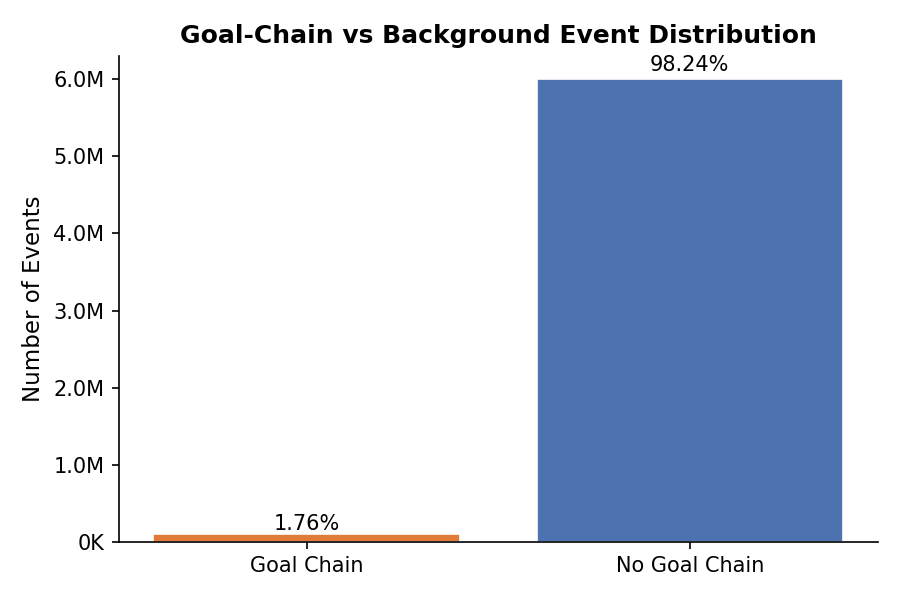
\includegraphics[width=0.7\textwidth]{../figures/eda_class_balance.png}
    \caption{Distribution of goal-chain events versus background events in the Version 1 dataset. Only 1.76\% of events belong to a goal-scoring possession chain, reflecting the fundamental rarity of goals in football.}
    \label{fig:class_balance}
\end{figure}

\begin{figure}[h]
    \centering
    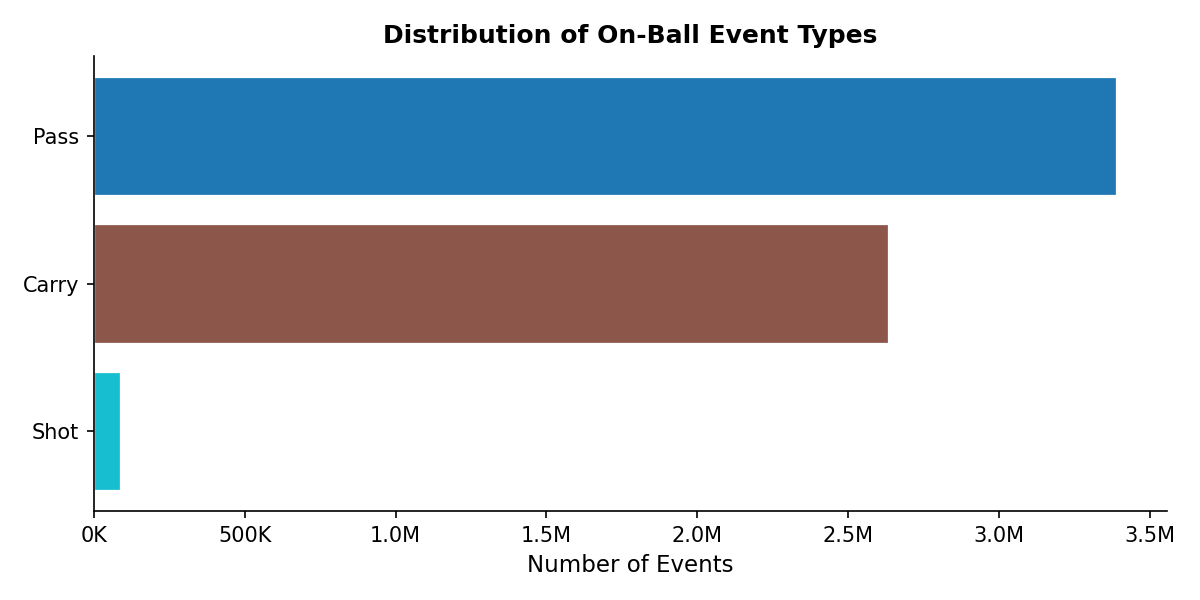
\includegraphics[width=0.85\textwidth]{../figures/eda_event_types.png}
    \caption{Distribution of on-ball event types in the Version 1 dataset. Passes account for the largest share, with shots constituting a small fraction of total events.}
    \label{fig:event_types}
\end{figure}

\begin{figure}[h]
    \centering
    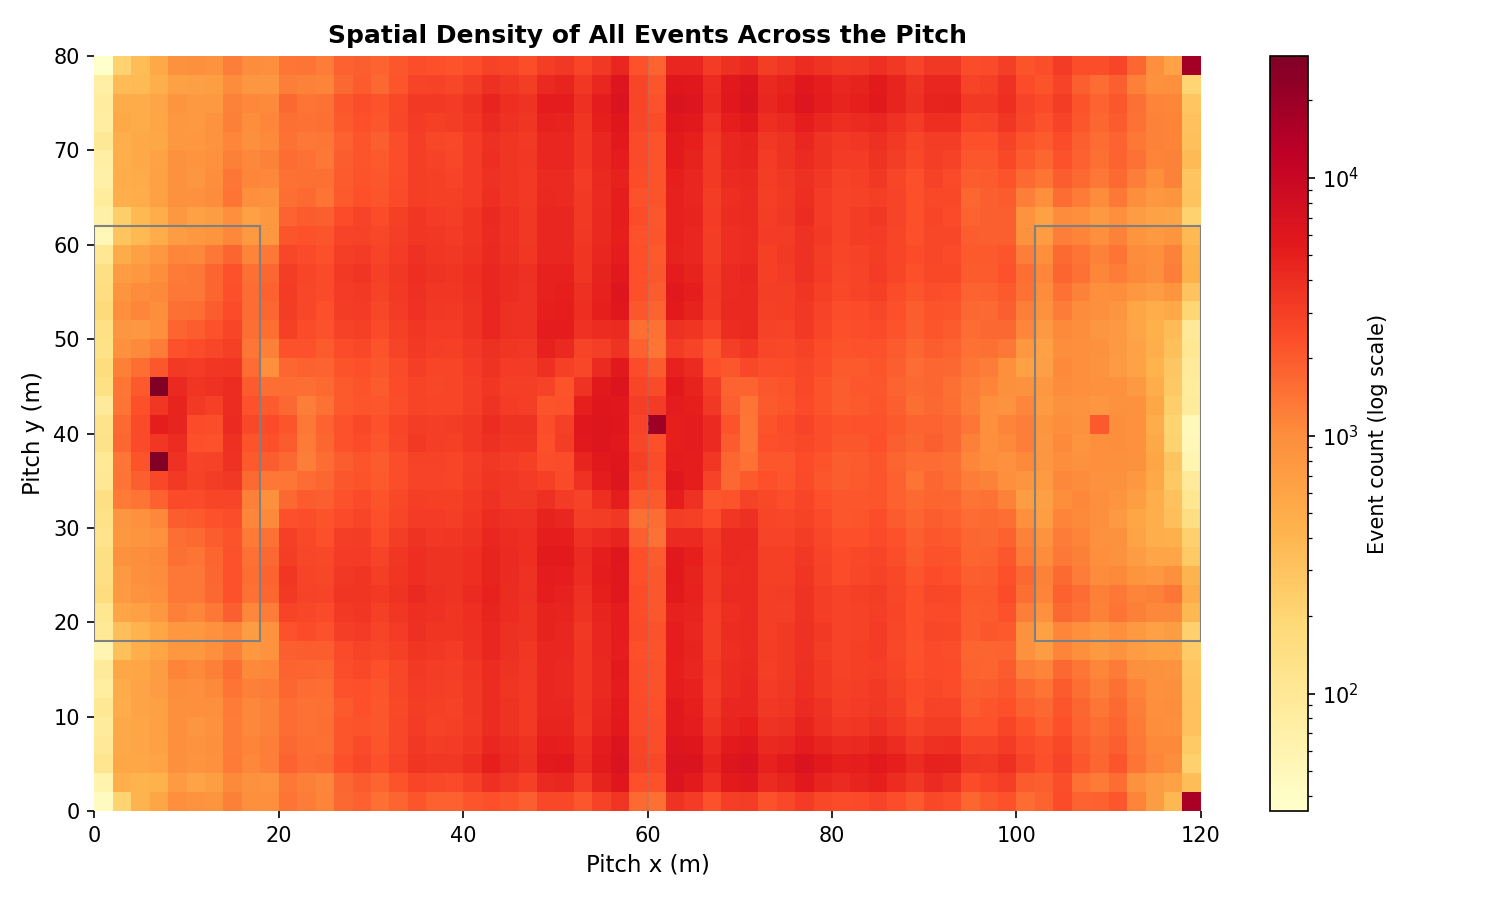
\includegraphics[width=0.85\textwidth]{../figures/eda_spatial_density.png}
    \caption{Spatial density of all events across the pitch (Version 1 dataset). Darker regions indicate higher event frequency. Activity is concentrated in central areas with a secondary cluster around the attacking penalty area.}
    \label{fig:spatial_density}
\end{figure}

\begin{figure}[h]
    \centering
    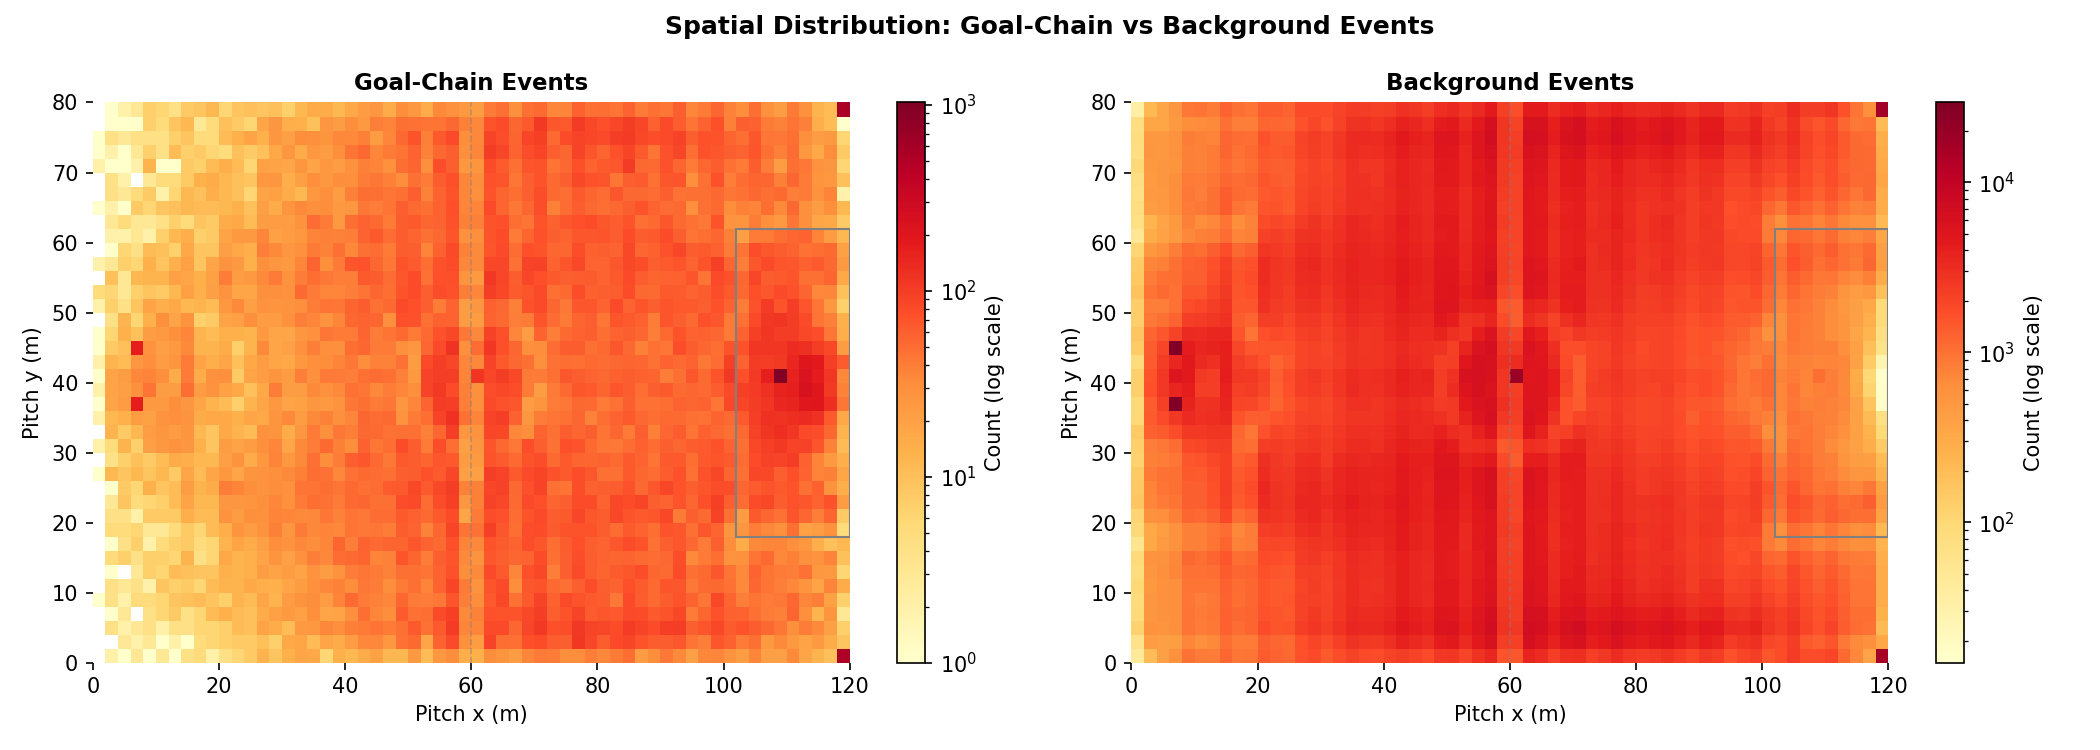
\includegraphics[width=0.85\textwidth]{../figures/eda_goal_chain_locs.png}
    \caption{Spatial distribution of goal-chain events (left) versus background events (right). Goal-chain events are strongly concentrated near the attacking goal, confirming that distance to goal is the primary predictor of threat.}
    \label{fig:goal_chain_locs}
\end{figure}

\begin{figure}[h]
    \centering
    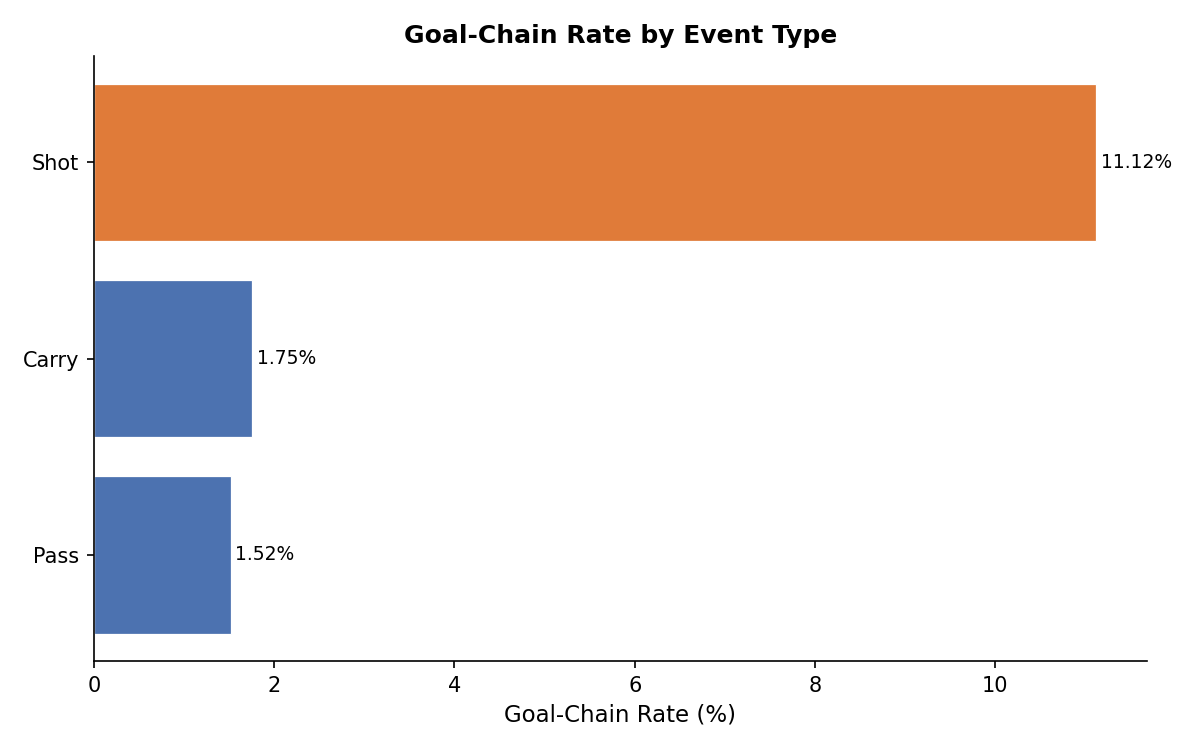
\includegraphics[width=0.8\textwidth]{../figures/eda_goal_rate_by_type.png}
    \caption{Goal-chain rate per event type. Shots dominate; and carries show the highest rates among non-shot actions.}
    \label{fig:goal_rate_type}
\end{figure}

\begin{figure}[h]
    \centering
    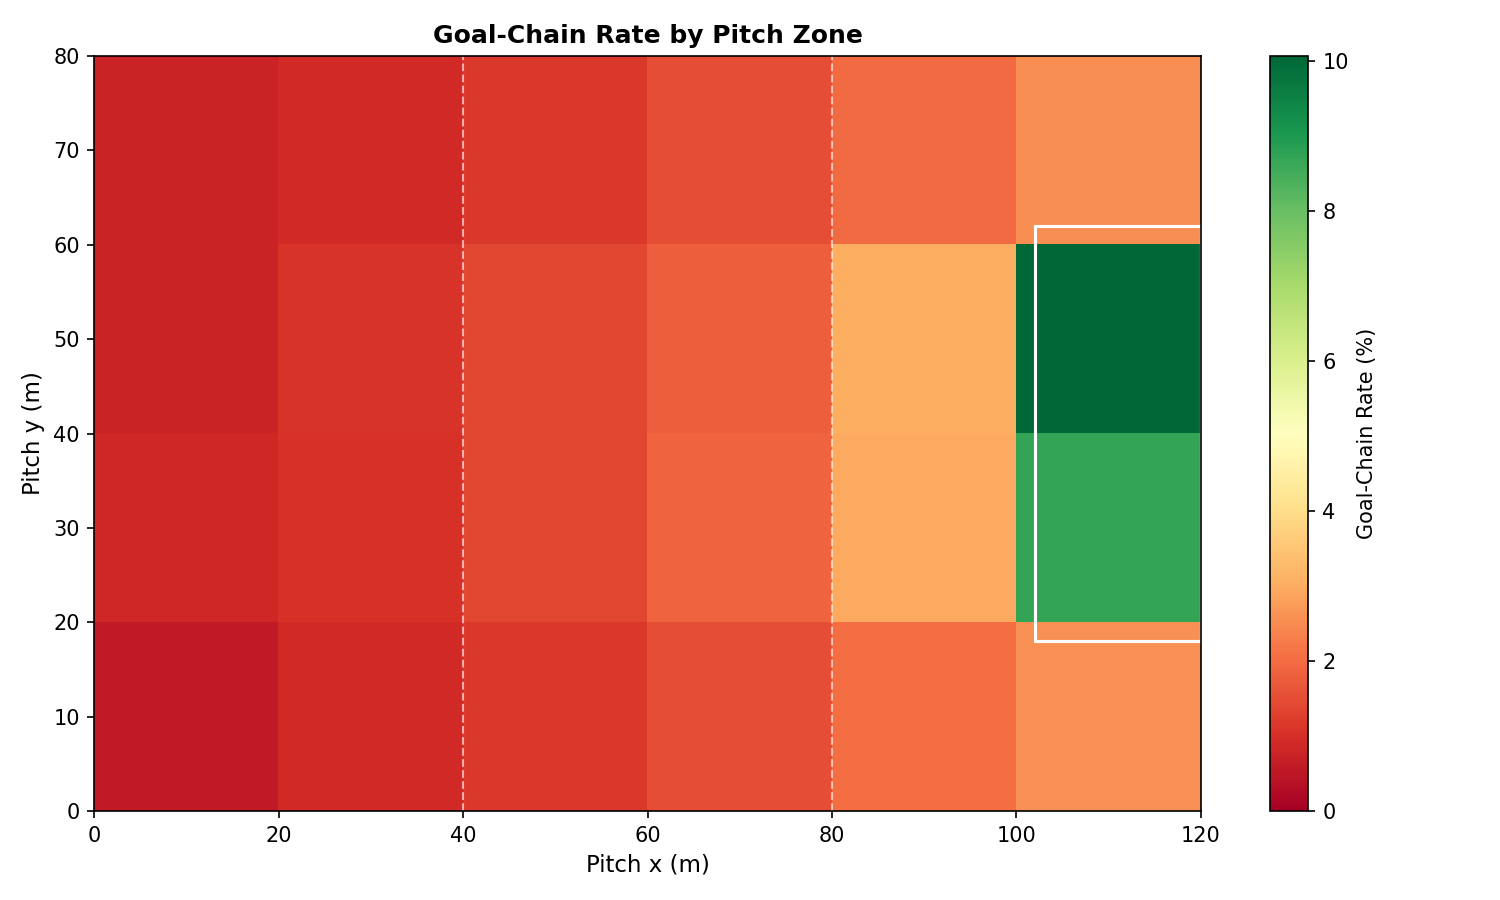
\includegraphics[width=0.85\textwidth]{../figures/eda_goal_rate_by_zone.png}
    \caption{Goal-chain rate by pitch zone. The attacking penalty area shows the highest rates, confirming spatial position as the dominant predictor of threat.}
    \label{fig:goal_rate_zone}
\end{figure}

\begin{figure}[h]
    \centering
    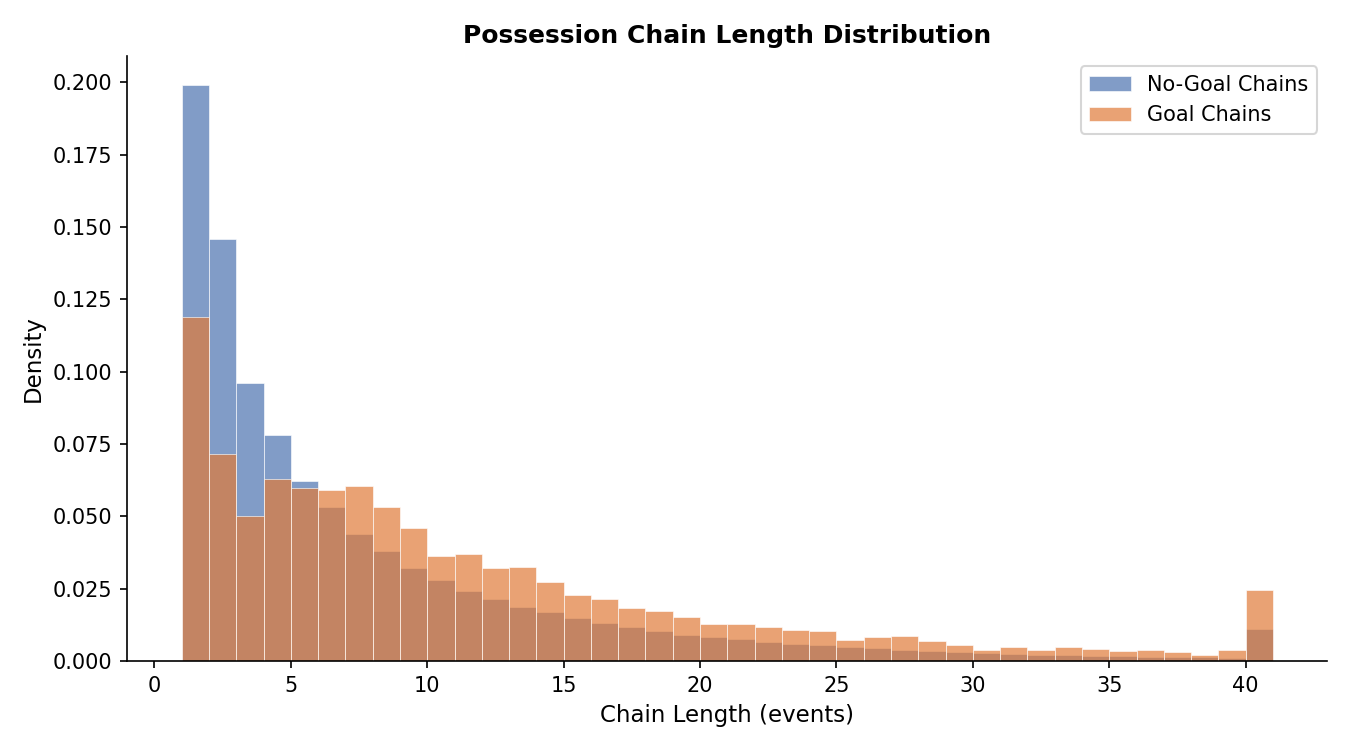
\includegraphics[width=0.8\textwidth]{../figures/eda_chain_lengths.png}
    \caption{Possession chain length distribution for goal-scoring and background chains. Goal chains are typically shorter and more direct.}
    \label{fig:chain_lengths}
\end{figure}

\begin{figure}[h]
    \centering
    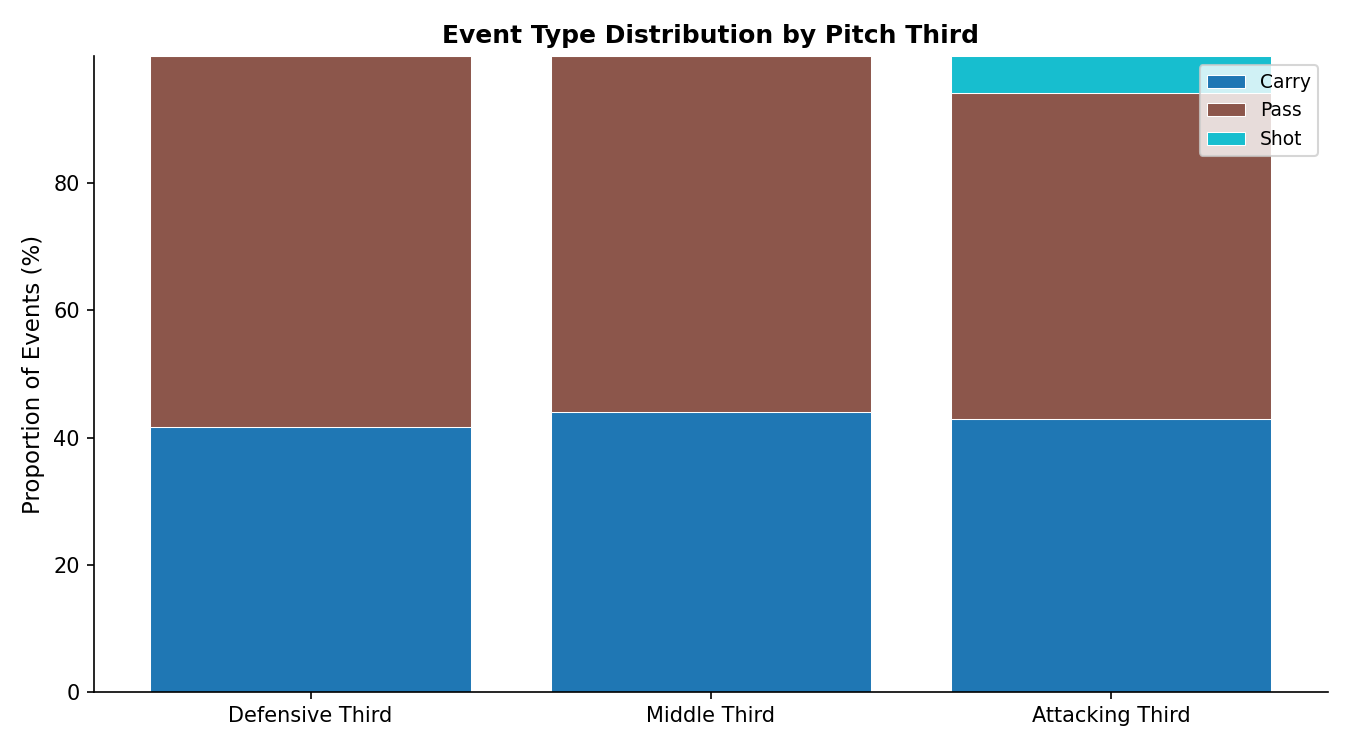
\includegraphics[width=0.85\textwidth]{../figures/eda_action_by_third.png}
    \caption{Proportion of each event type within the defensive, middle, and attacking thirds.}
    \label{fig:action_by_third}
\end{figure}

\begin{figure}[h]
    \centering
    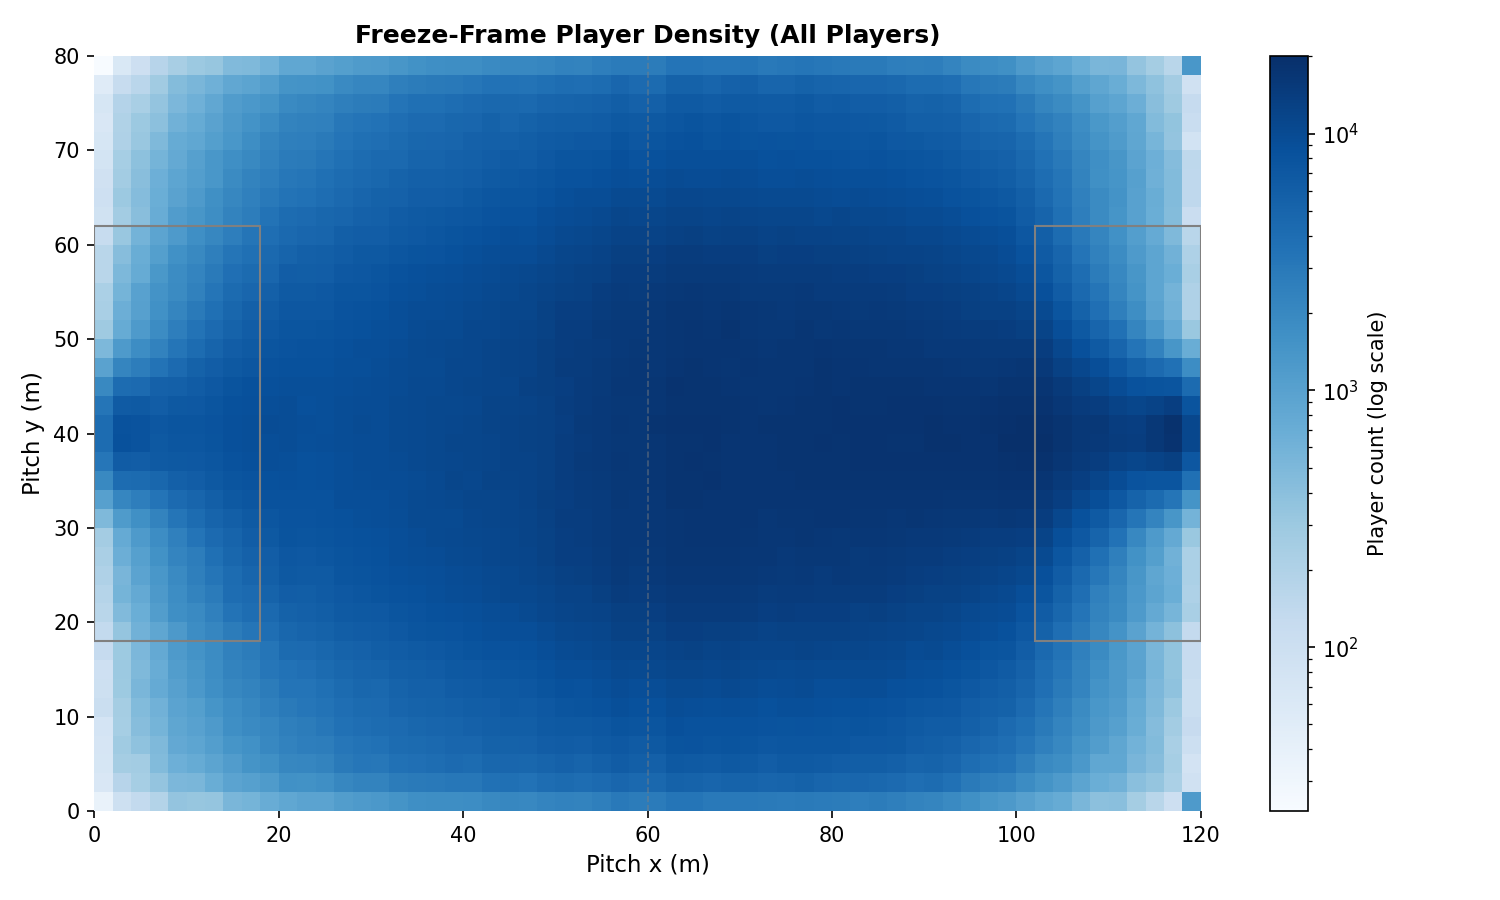
\includegraphics[width=0.85\textwidth]{../figures/eda_player_density.png}
    \caption{Spatial density of all player positions in 360 freeze frames (log scale). Players concentrate around the ball and in central corridors.}
    \label{fig:player_density}
\end{figure}

\begin{figure}[h]
    \centering
    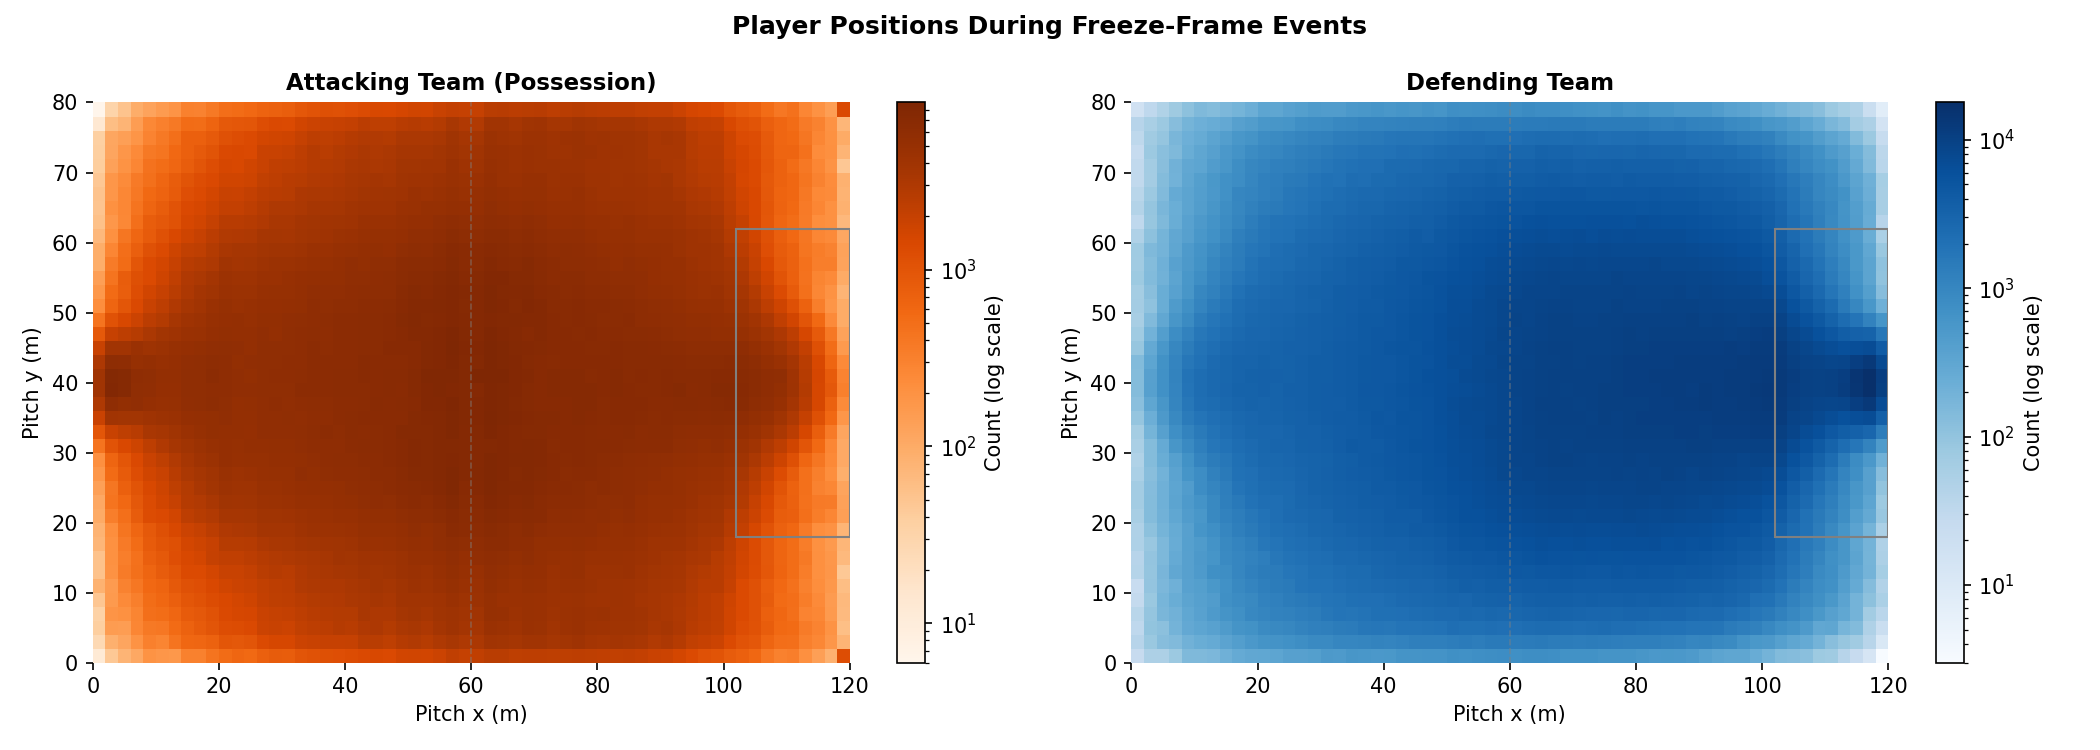
\includegraphics[width=\textwidth]{../figures/eda_team_positions.png}
    \caption{Freeze-frame player positions split by attacking team (left) and defending team (right). The teams occupy clearly distinct regions of the pitch.}
    \label{fig:team_positions}
\end{figure}

\begin{figure}[h]
    \centering
    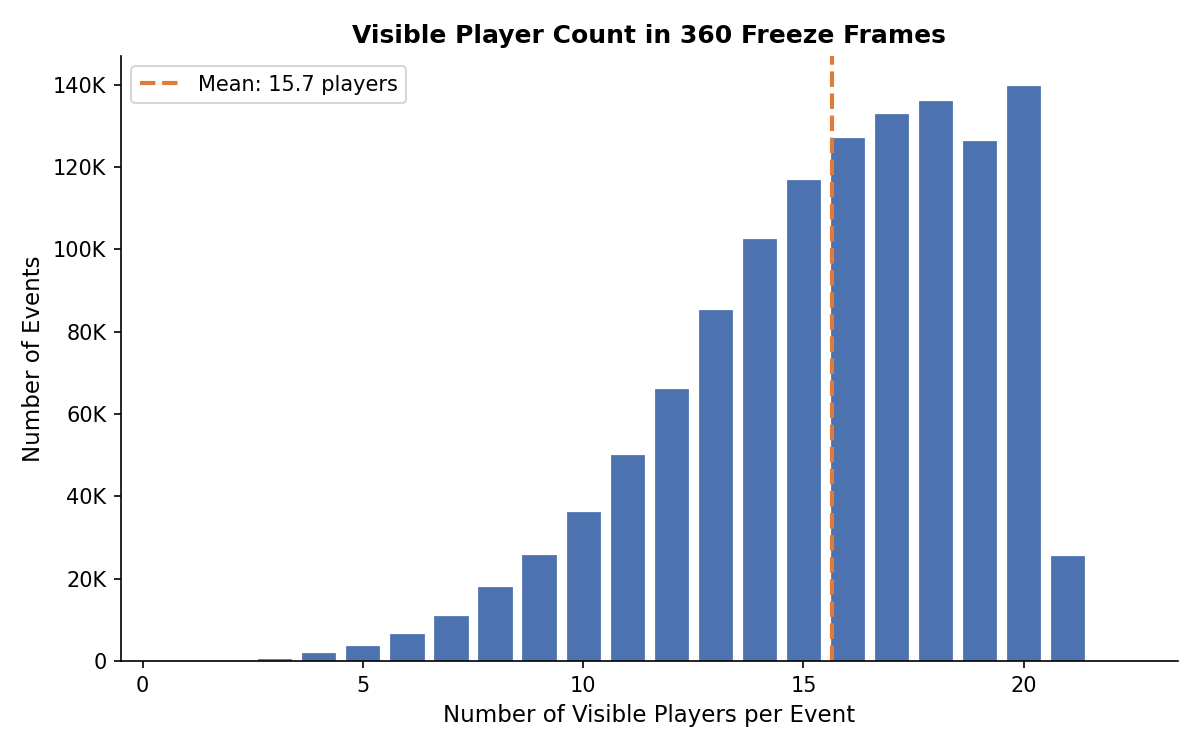
\includegraphics[width=0.7\textwidth]{../figures/eda_player_count.png}
    \caption{Distribution of visible player counts per freeze-frame event. Most events capture near-complete player information, validating the 360 data as a reliable source of positional context.}
    \label{fig:player_count}
\end{figure}

\clearpage

\section{Feature Correlation}

\begin{figure}[h]
    \centering
    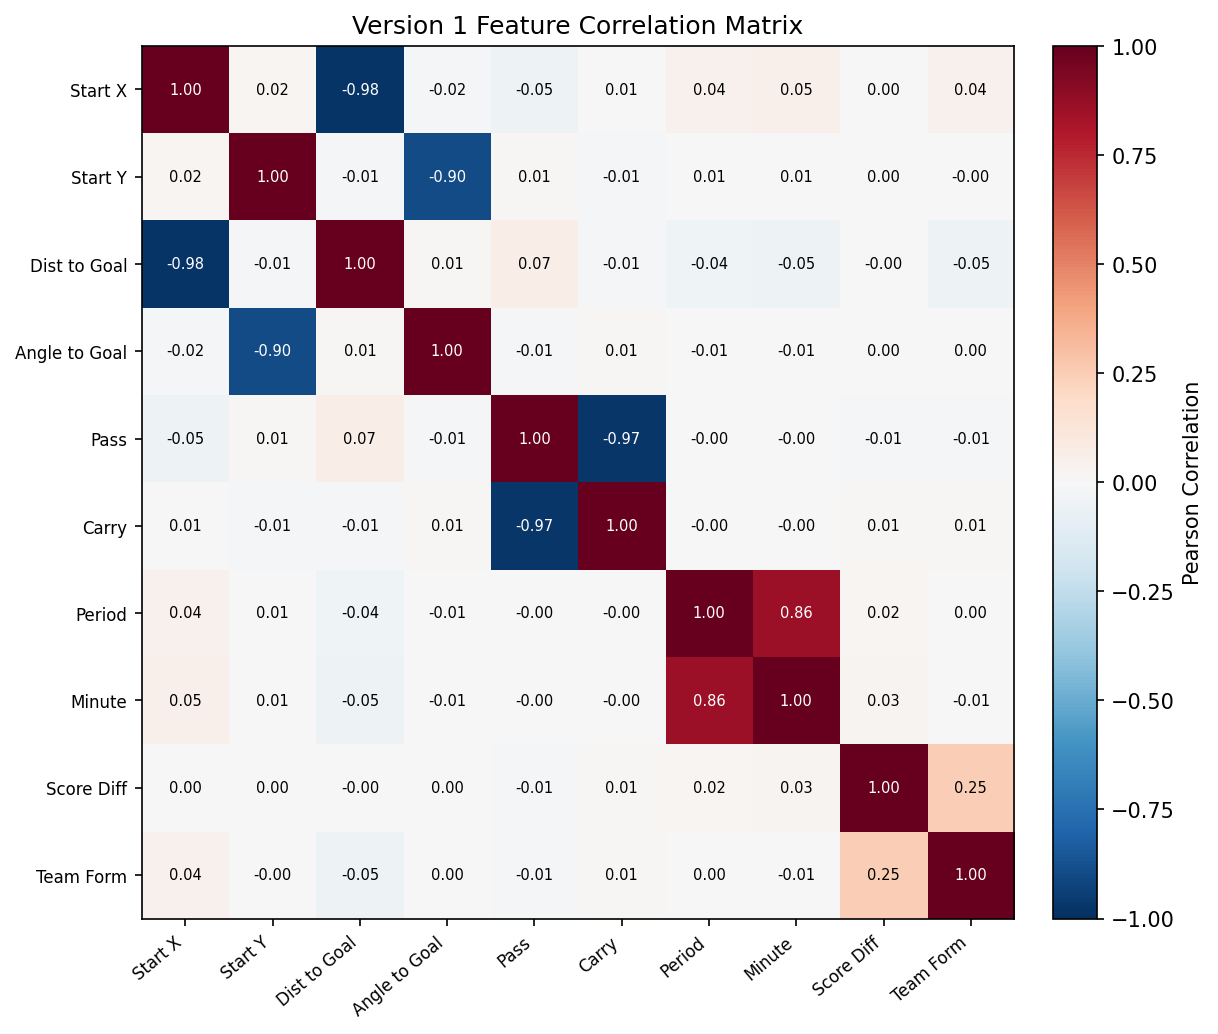
\includegraphics[width=0.72\textwidth]{../xT_v1/xt_feature_correlation.png}
    \caption{Pearson correlation matrix for Version 1 input features.}
    \label{fig:feat_corr}
\end{figure}

\clearpage

\section{Version 1: Random Forest}

\begin{figure}[h]
    \centering
    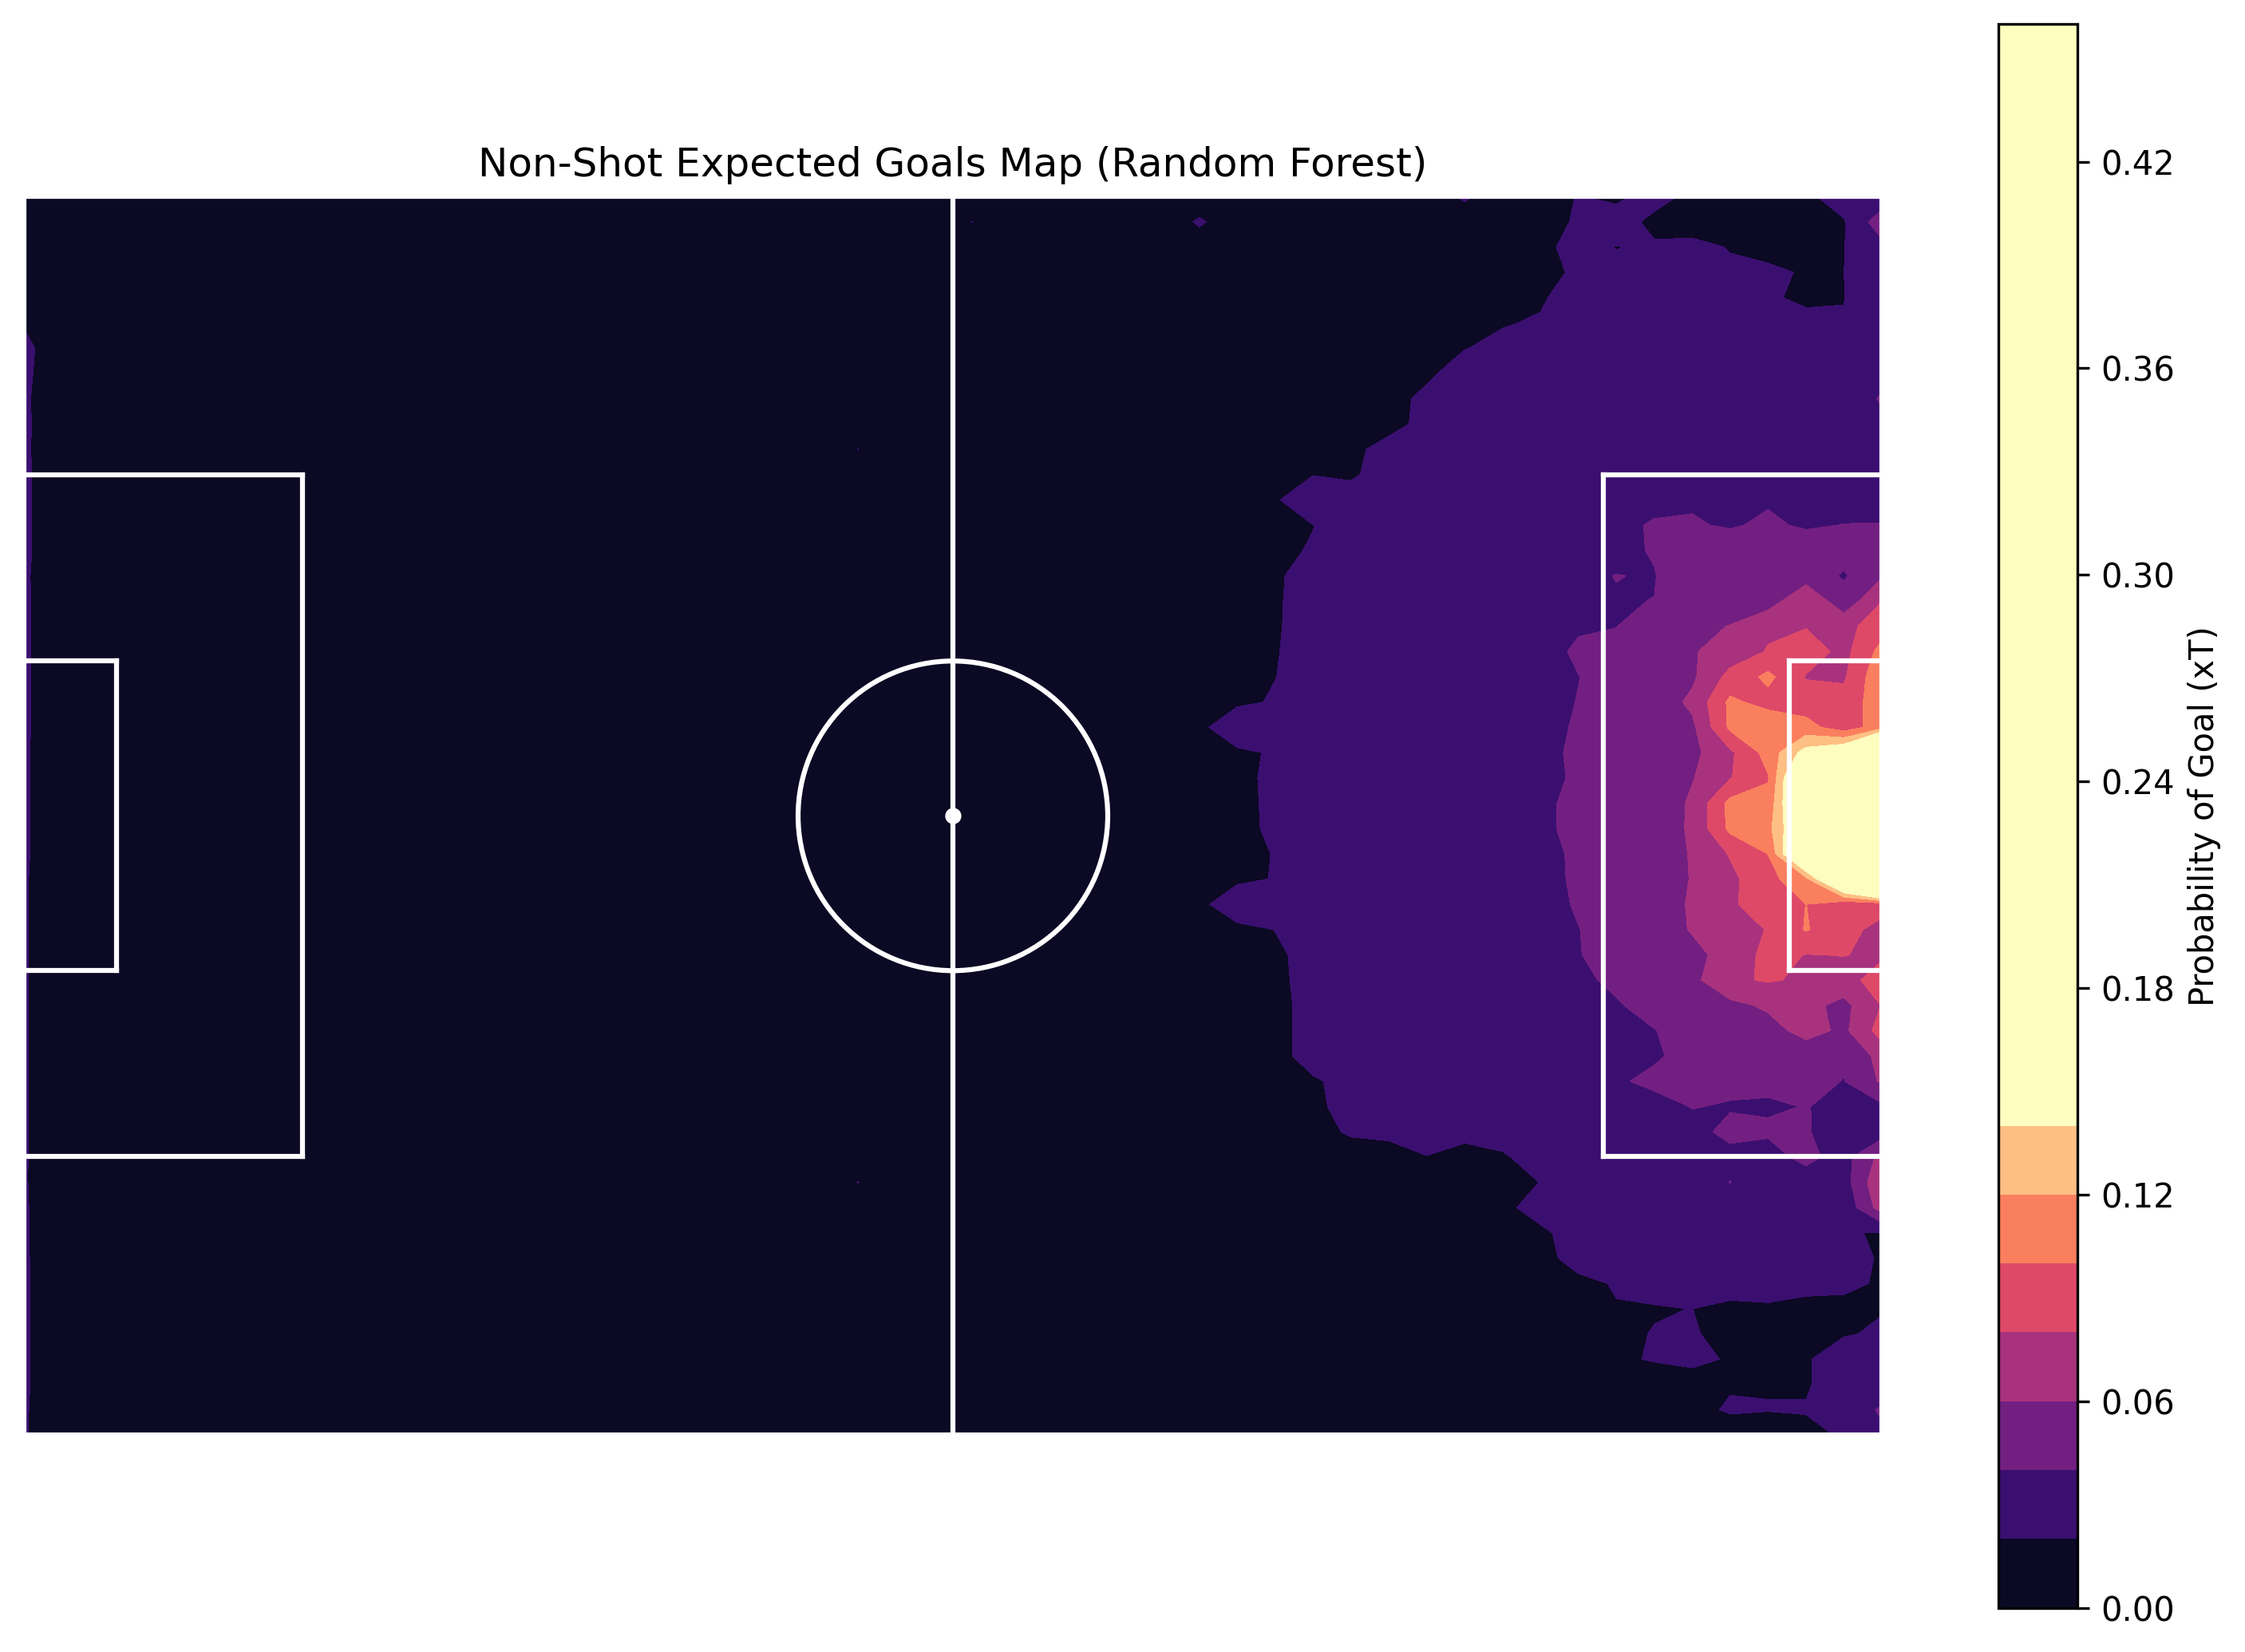
\includegraphics[width=0.8\textwidth]{../xT_v1/xt_heatmap.png}
    \caption{SxT heatmap for Version 1 (Random Forest), generated by querying the model at every grid cell assuming a Pass action type at a neutral game state (period 2, minute 45, score level, average team form). See Appendix~\ref{app:metrics} for full metric tables.}
    \label{fig:v1_heatmap}
\end{figure}

\begin{figure}[h]
    \centering
    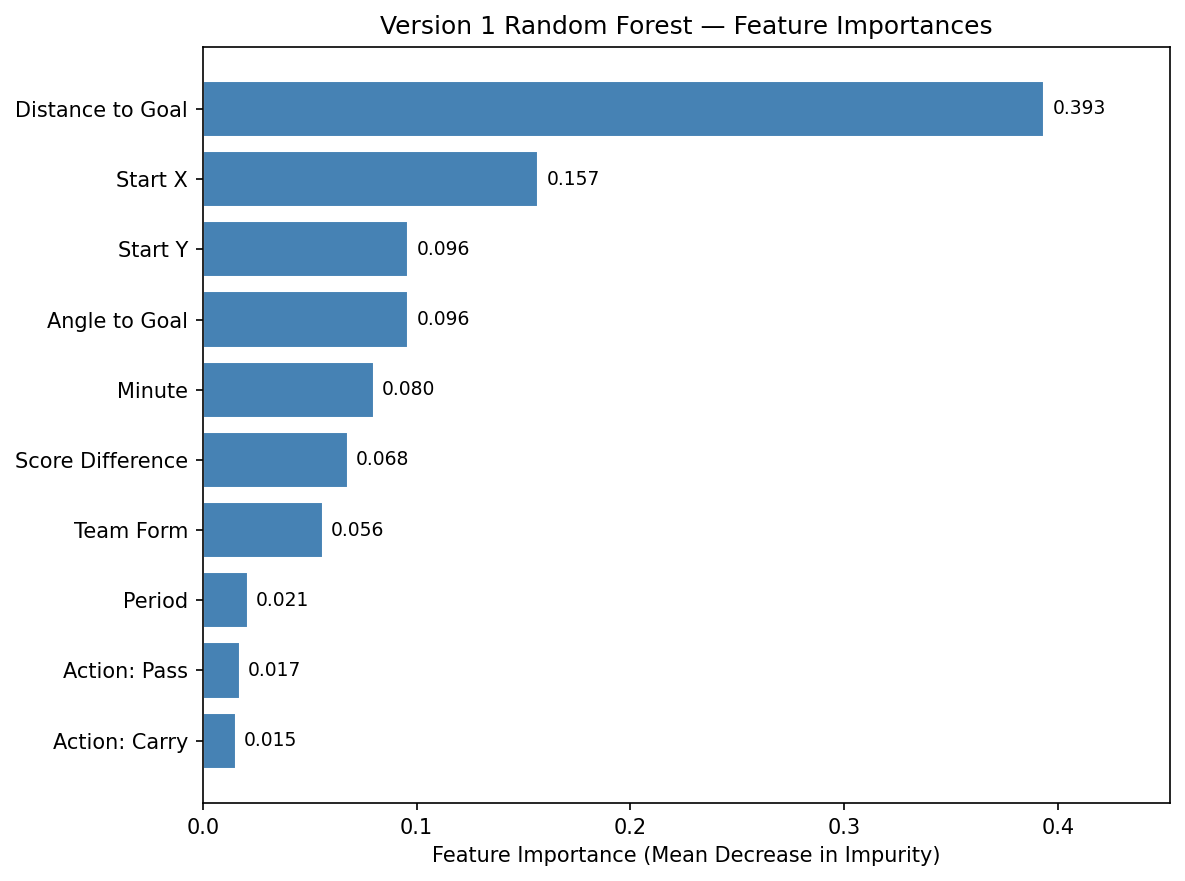
\includegraphics[width=0.85\textwidth]{../xT_v1/xt_feature_importance.png}
    \caption{Feature importance scores for the Version 1 Random Forest (mean decrease in impurity).}
    \label{fig:v1_importance}
\end{figure}

\clearpage

\section{Version 2: CNN + MLP}

\begin{figure}[h]
\centering
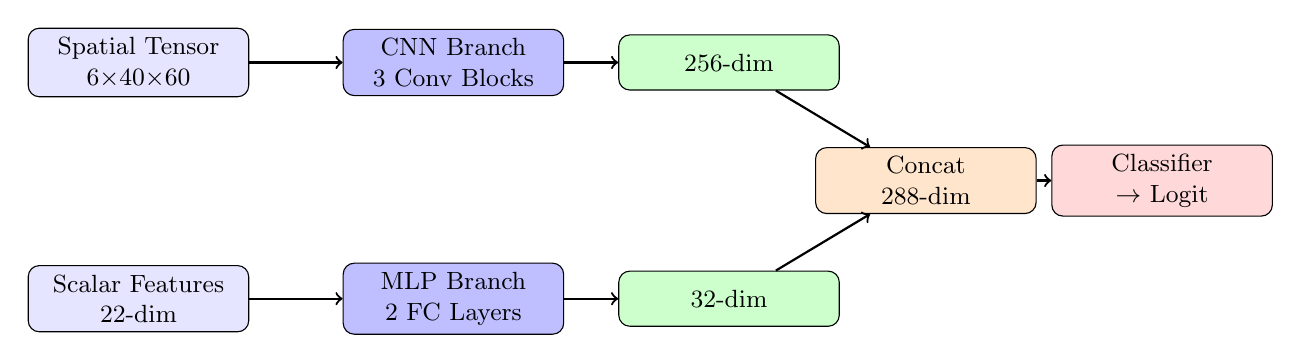
\begin{tikzpicture}[
    box/.style={draw, rounded corners, minimum width=2.8cm, minimum height=0.7cm, align=center, font=\small},
    arr/.style={->, thick}
]
\node[box, fill=blue!10]  (spatial) at (0, 3)    {Spatial Tensor\\$6{\times}40{\times}60$};
\node[box, fill=blue!10]  (scalar)  at (0, 0)    {Scalar Features\\$22$-dim};
\node[box, fill=blue!25]  (cnn)     at (4, 3)    {CNN Branch\\3 Conv Blocks};
\node[box, fill=blue!25]  (mlp)     at (4, 0)    {MLP Branch\\2 FC Layers};
\node[box, fill=green!20] (cnnout)  at (7.5, 3)  {256-dim};
\node[box, fill=green!20] (mlpout)  at (7.5, 0)  {32-dim};
\node[box, fill=orange!20](concat)  at (10, 1.5) {Concat\\288-dim};
\node[box, fill=red!15]   (cls)     at (13, 1.5) {Classifier\\$\to$ Logit};

\draw[arr] (spatial) -- (cnn);
\draw[arr] (scalar)  -- (mlp);
\draw[arr] (cnn)     -- (cnnout);
\draw[arr] (mlp)     -- (mlpout);
\draw[arr] (cnnout)  -- (concat);
\draw[arr] (mlpout)  -- (concat);
\draw[arr] (concat)  -- (cls);
\end{tikzpicture}
\caption{Version 2 dual-branch architecture. The CNN branch processes the spatial pitch tensor; the MLP branch processes scalar context features. Their outputs are concatenated and passed to a final classifier.}
\label{fig:v2arch}
\end{figure}

\begin{figure}[h]
    \centering
    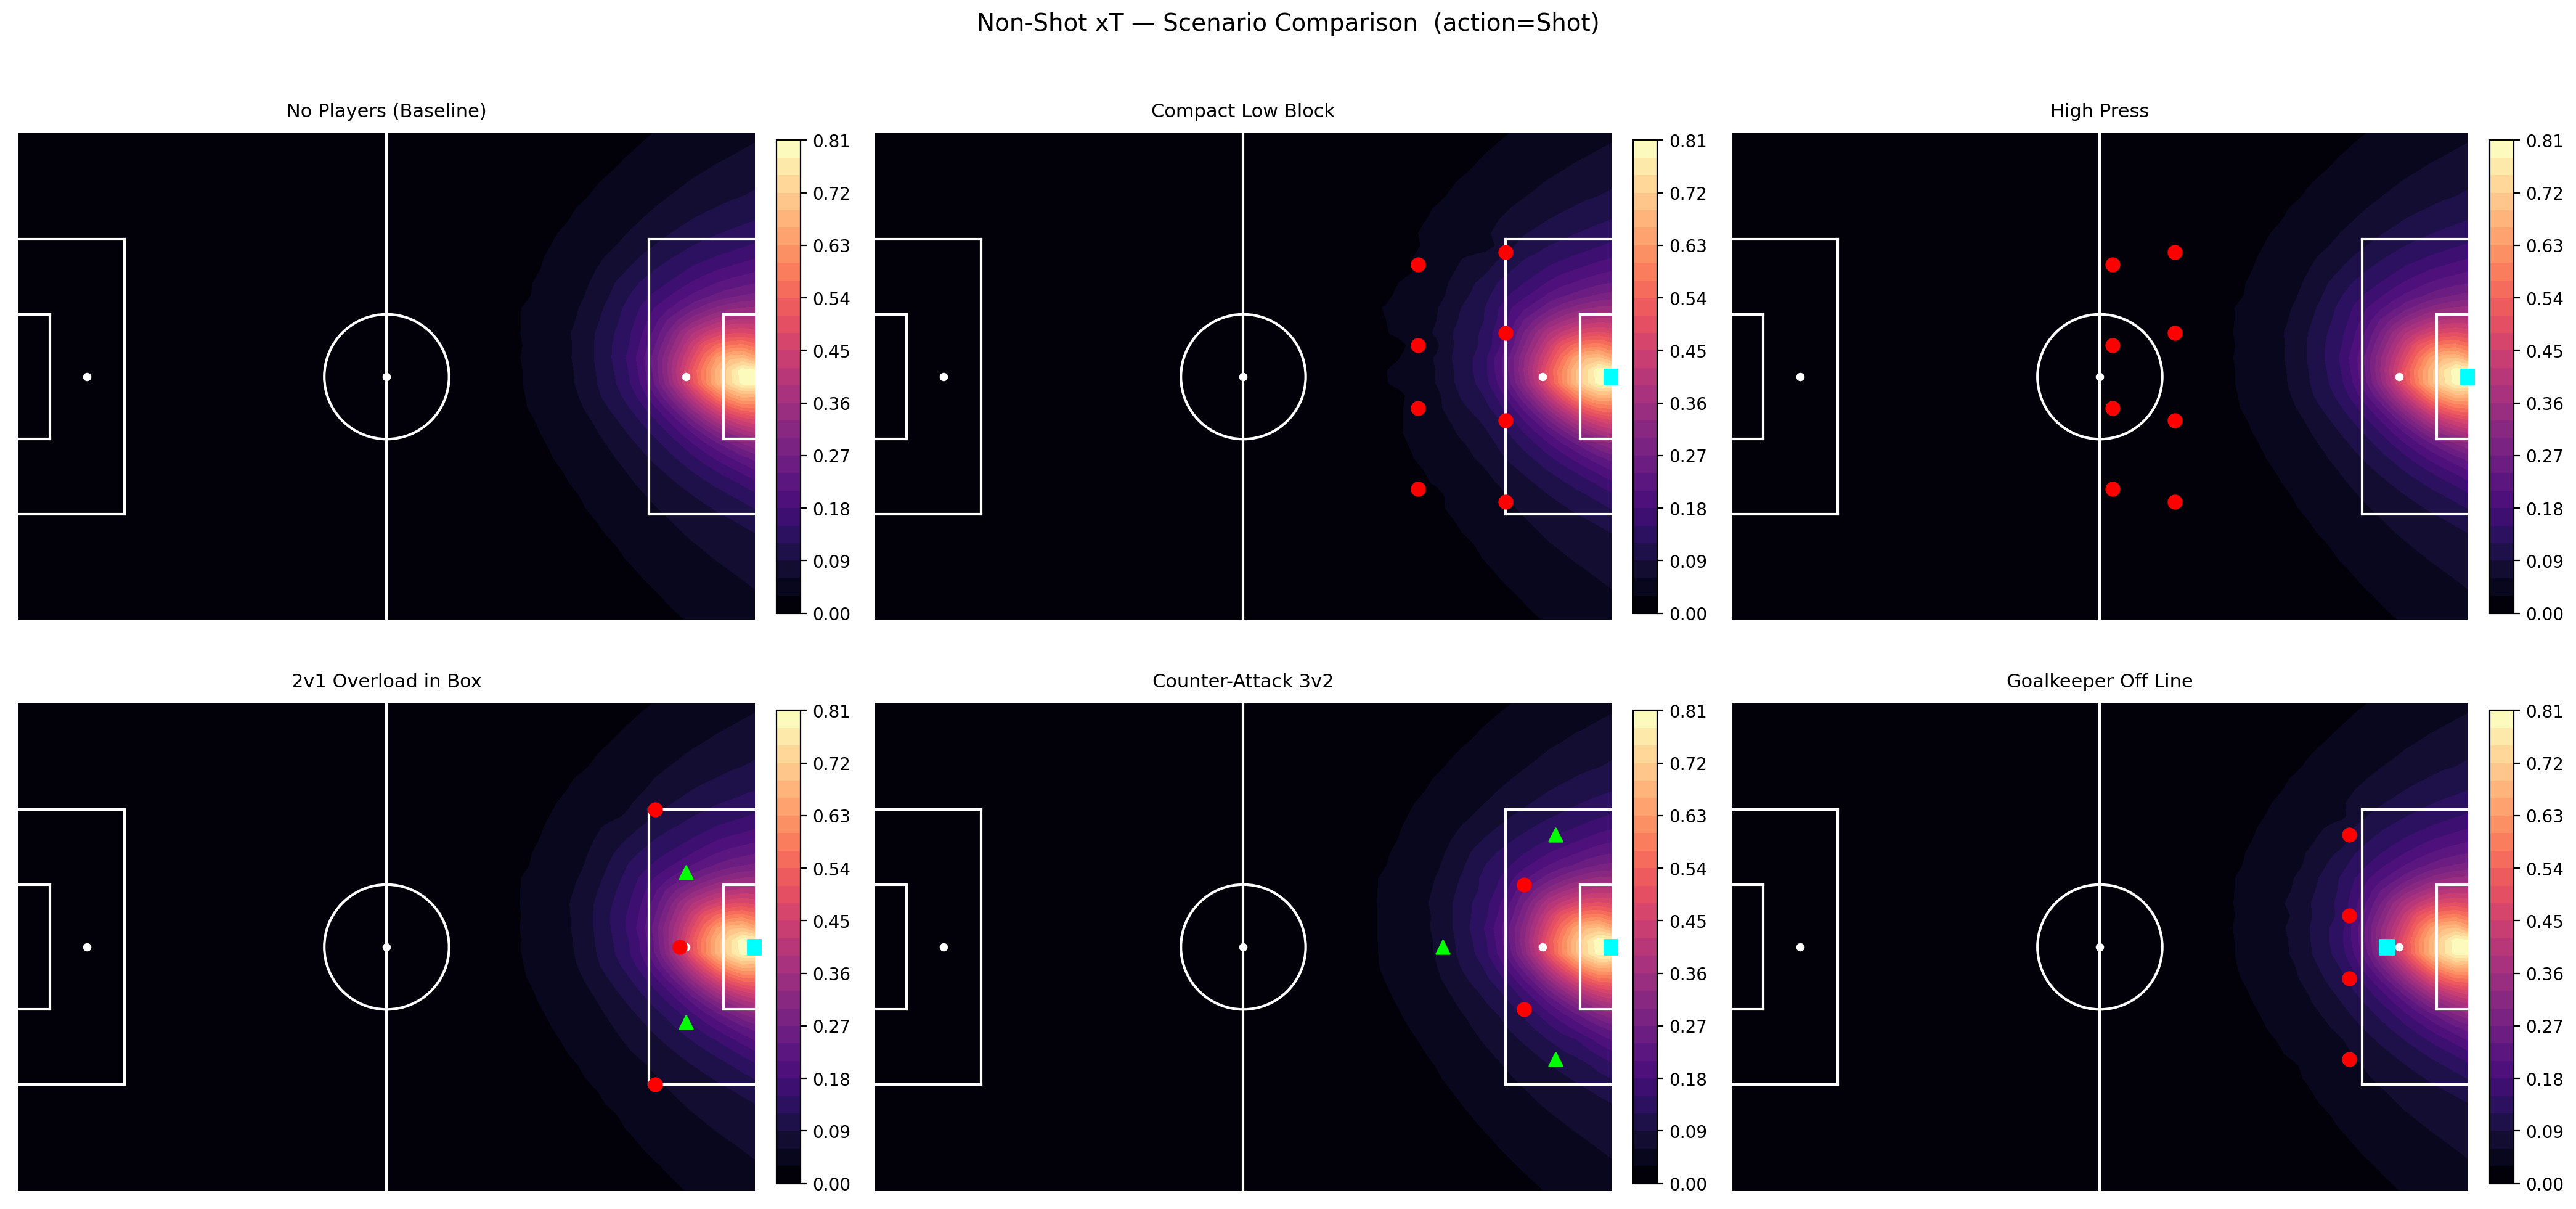
\includegraphics[width=0.8\textwidth]{../visualisations/xt_scenarios_shot_v2.png}
    \caption{Scenario comparison for Version 2, Shot action type. Six defensive configurations are shown under the same neutral game-state baseline (period 1, minute 0, score tied); the first panel (no players) serves as the positional reference. The near-identical surfaces across all panels illustrate the CNN's inability to distinguish between formations of equal density.}
    \label{fig:v2_scenarios}
\end{figure}

The following figures show Version 2 scenario grids for Pass, Carry, and Dribble. No standalone baseline heatmaps are shown; the \textit{No Players (Baseline)} panel in each grid already serves as the positional reference.

For Pass, the xT at each grid cell is computed by running the model once per outfield teammate in the scenario, using that teammate's position as the pass end-point, and taking the maximum xT over all targets. Panels without outfield teammates are shown as black (zero xT) by design: Pass xT is undefined without a specific target. Four of the six scenarios contain no teammates; only the 2v1 Overload and Counter-Attack panels show non-zero Pass threat. The same convention applies to the Version 3 grids in the following section.

\begin{figure}[h]
    \centering
    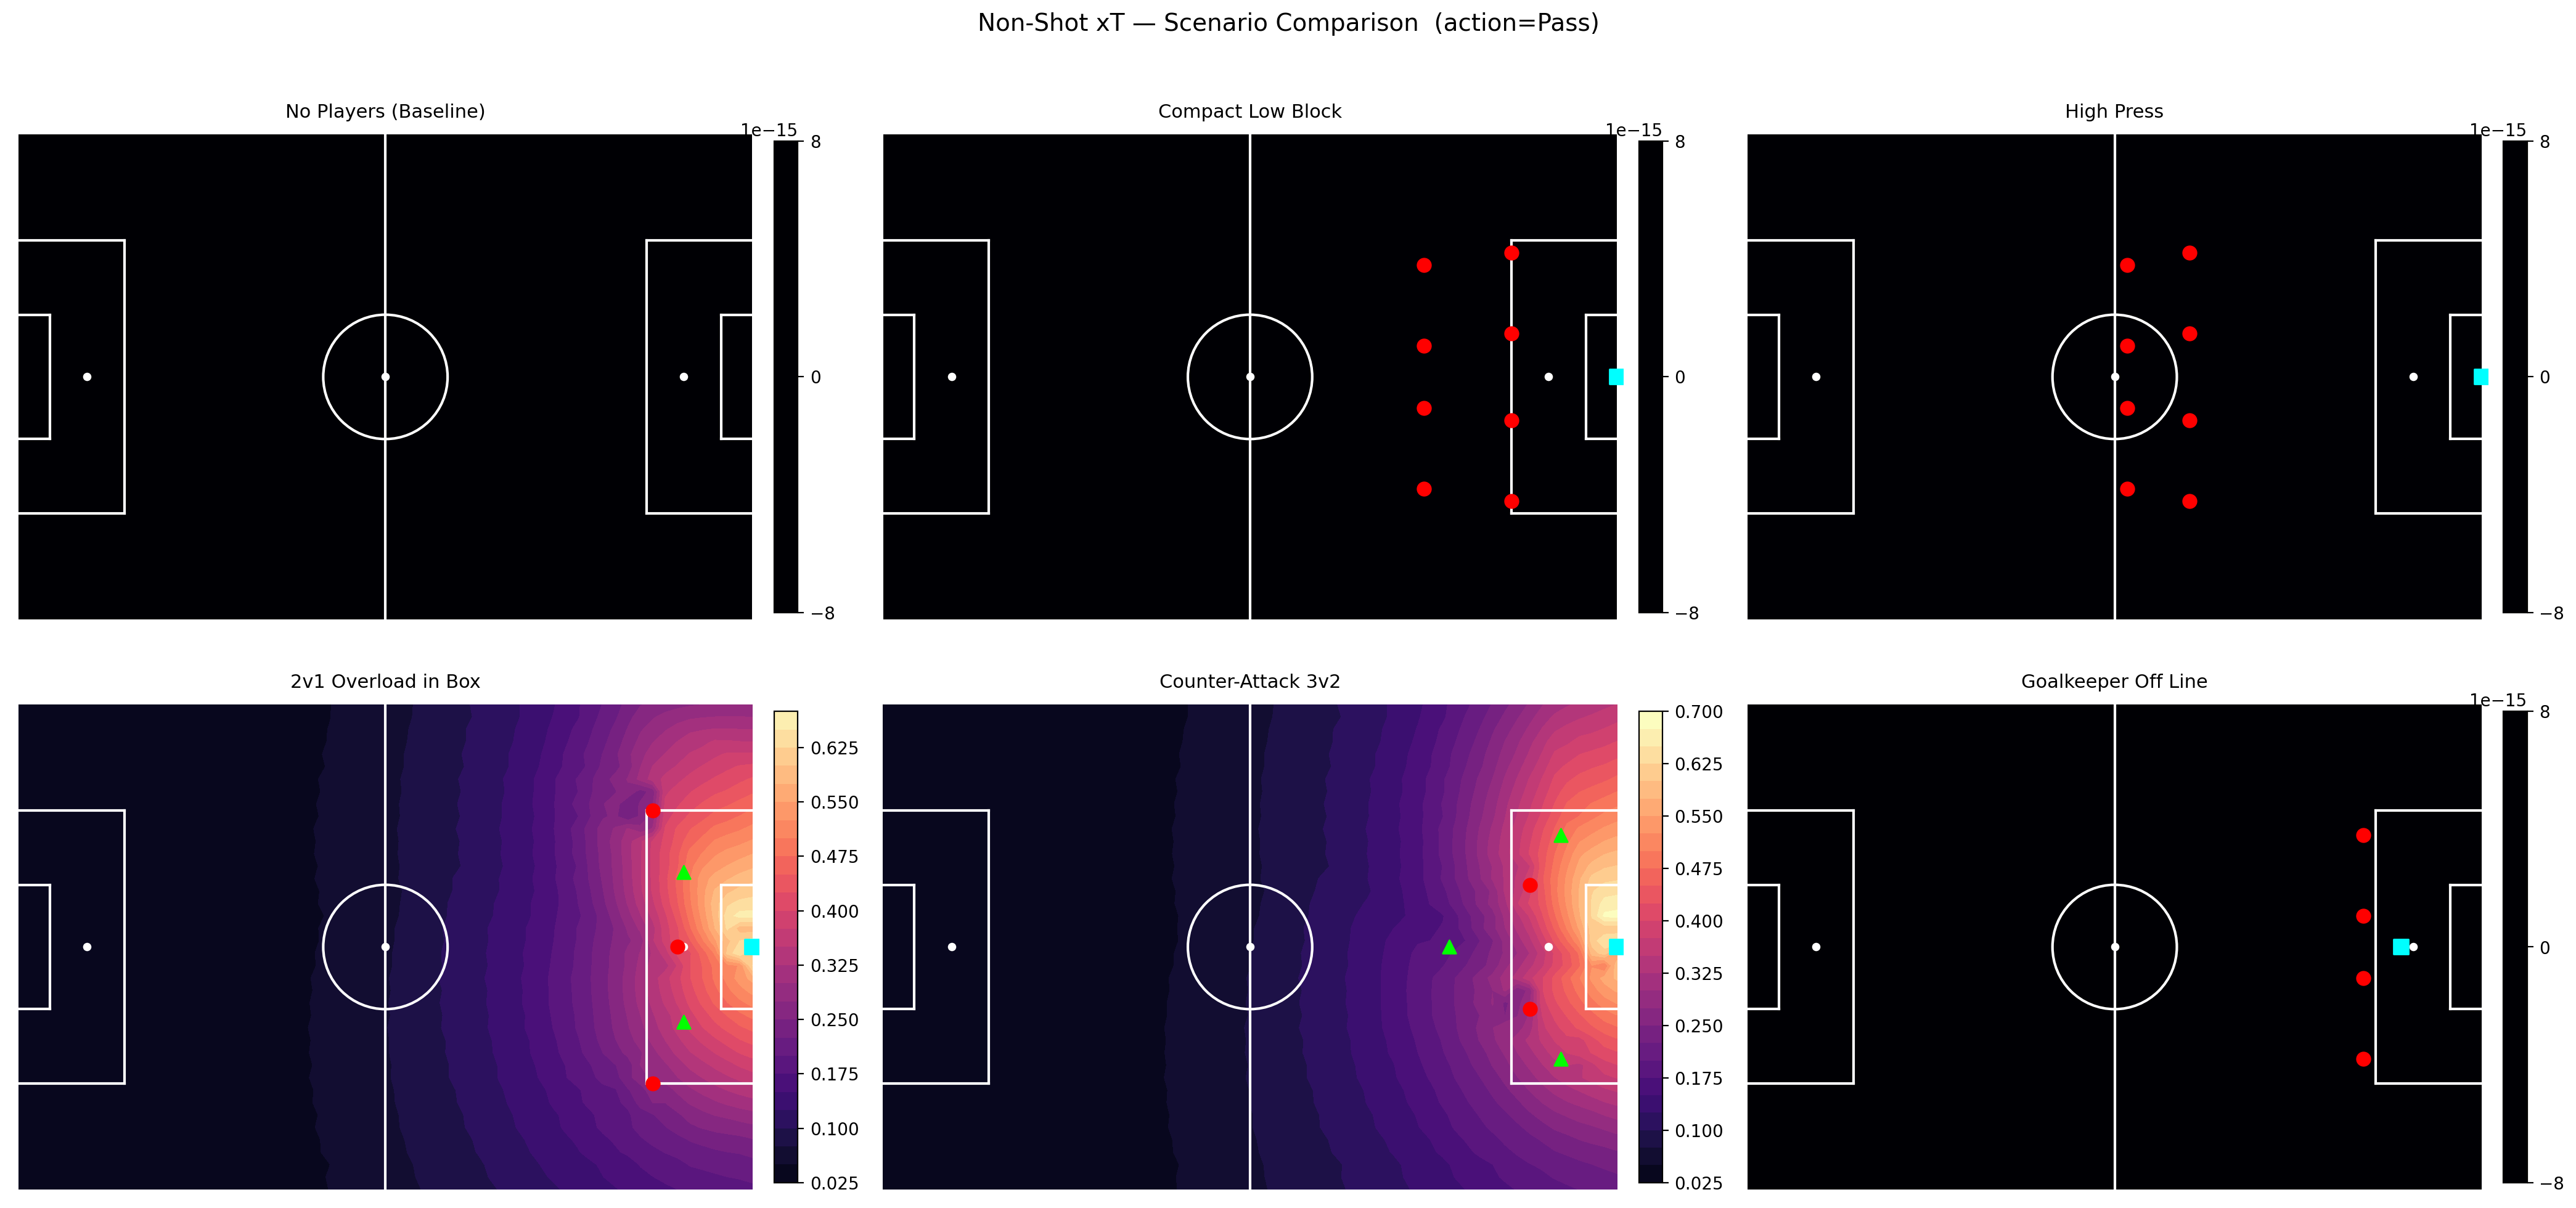
\includegraphics[width=0.8\textwidth]{../visualisations/xt_scenarios_pass_v2.png}
    \caption{Version 2 scenario comparison, Pass action type. Panels without outfield teammates are black --- Pass xT is zero when no target is available. The 2v1 Overload and Counter-Attack panels show non-zero threat reflecting passes to the positioned teammates. The CNN surfaces change little with formation, consistent with a density-based architecture.}
    \label{fig:v2_scenarios_pass}
\end{figure}

\begin{figure}[h]
    \centering
    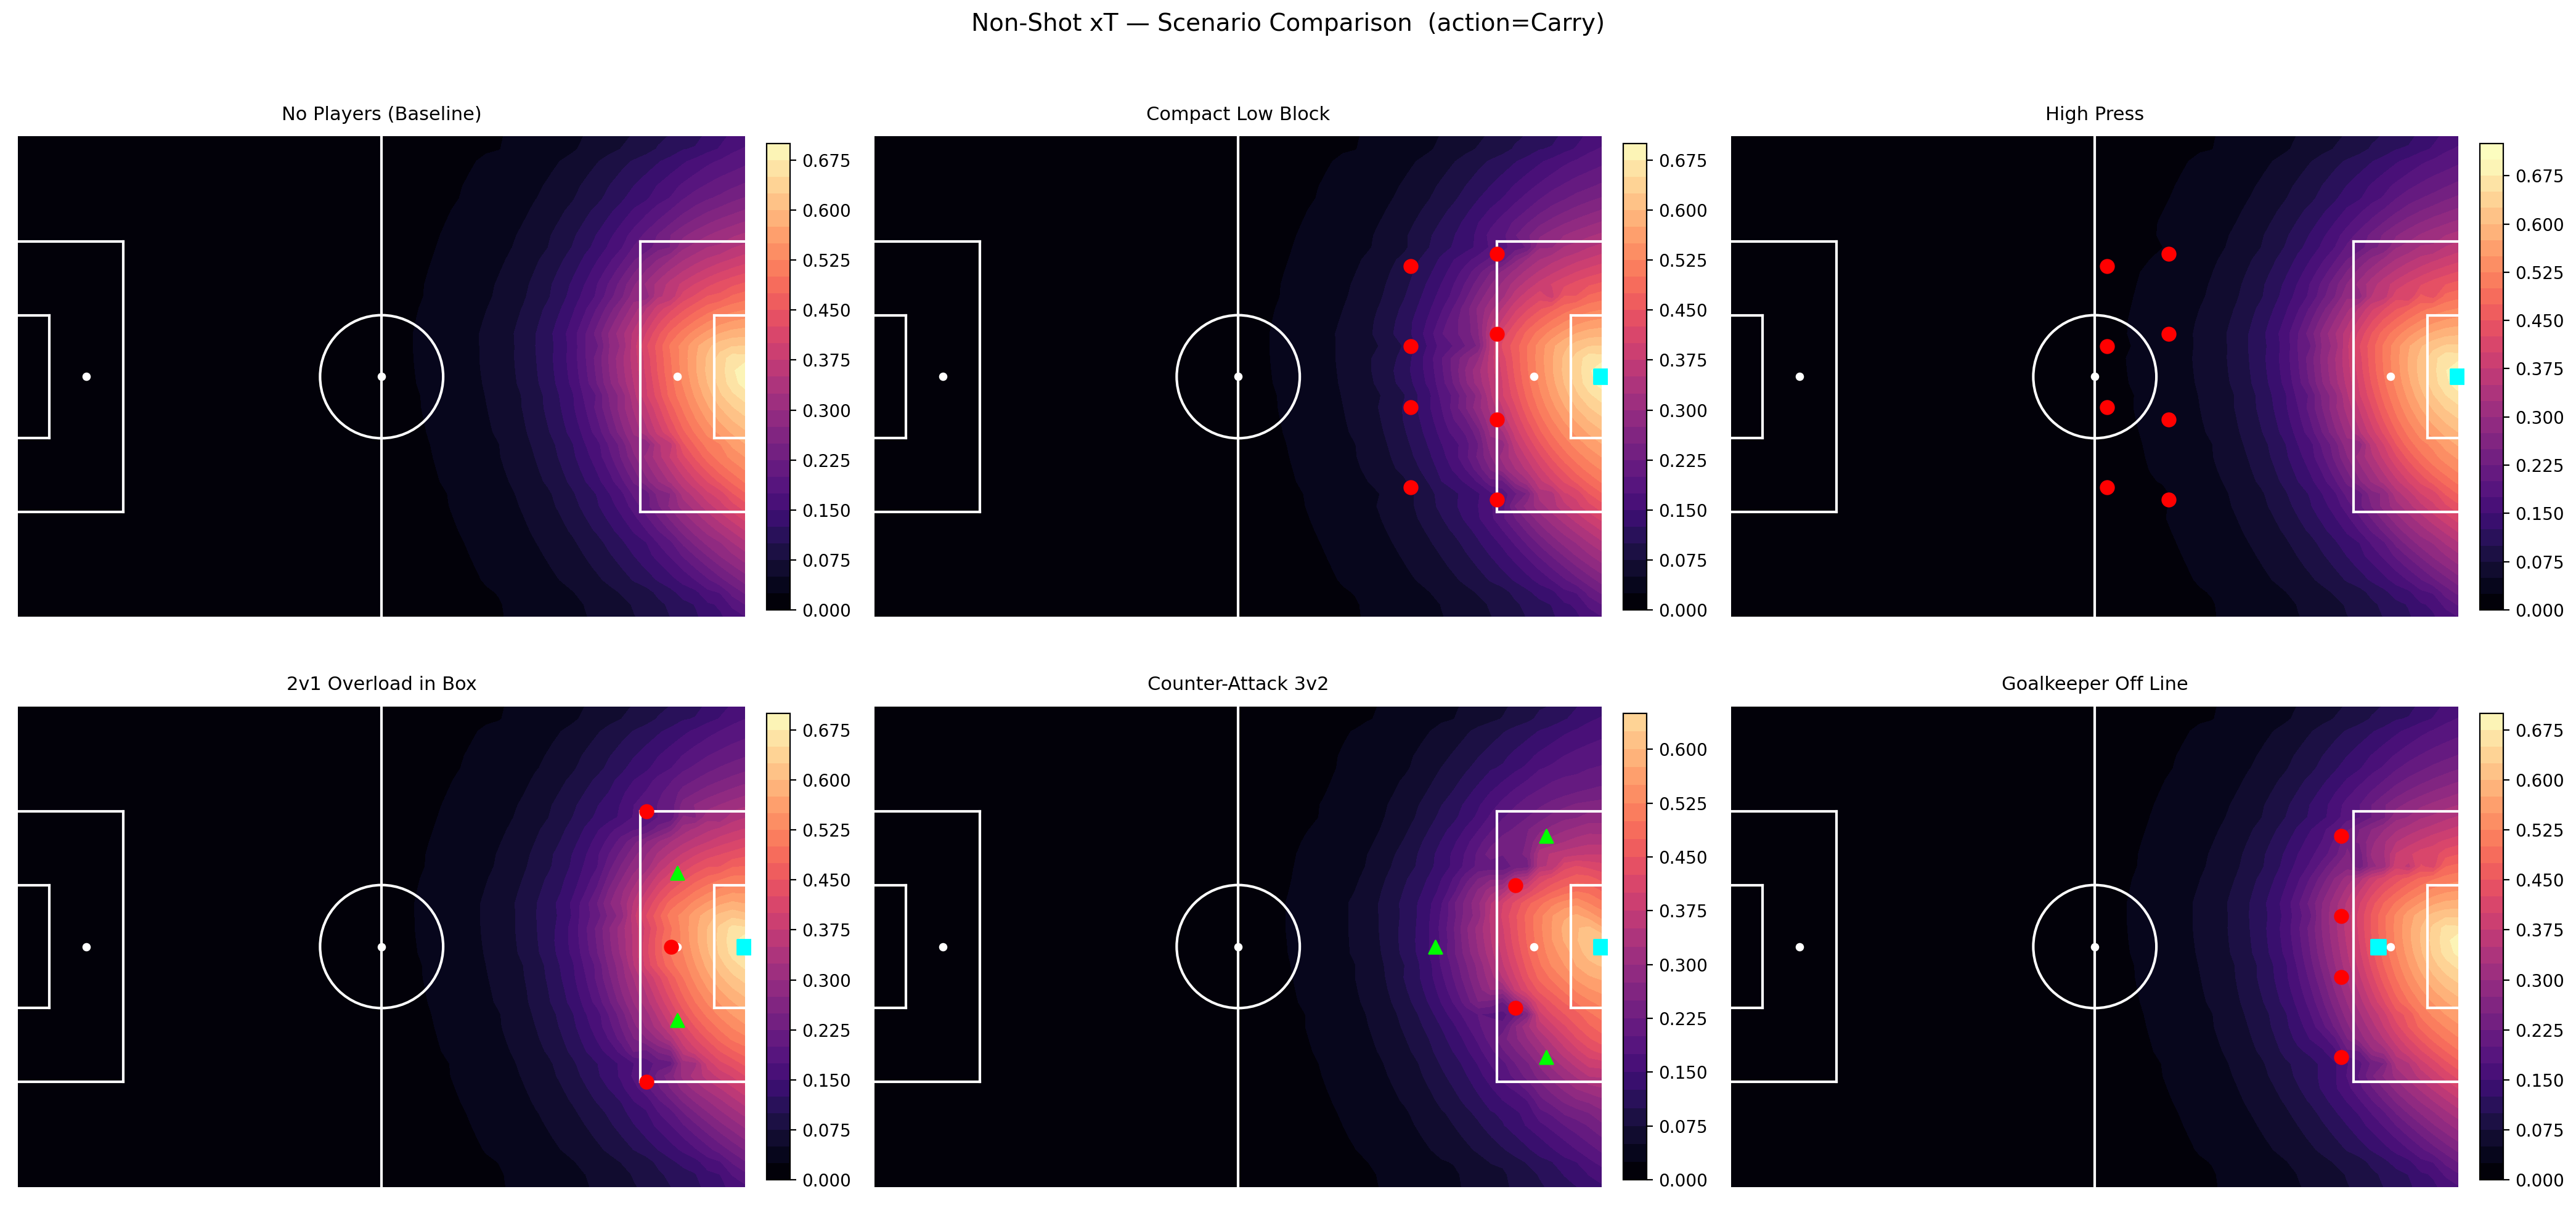
\includegraphics[width=0.8\textwidth]{../visualisations/xt_scenarios_carry_v2.png}
    \caption{Version 2 scenario comparison, Carry action type. End position is inferred as 8 yards toward goal from each cell. Surfaces are near-identical across formations, confirming the CNN's inability to distinguish between defensive configurations of equal density.}
    \label{fig:v2_scenarios_carry}
\end{figure}

\begin{figure}[h]
    \centering
    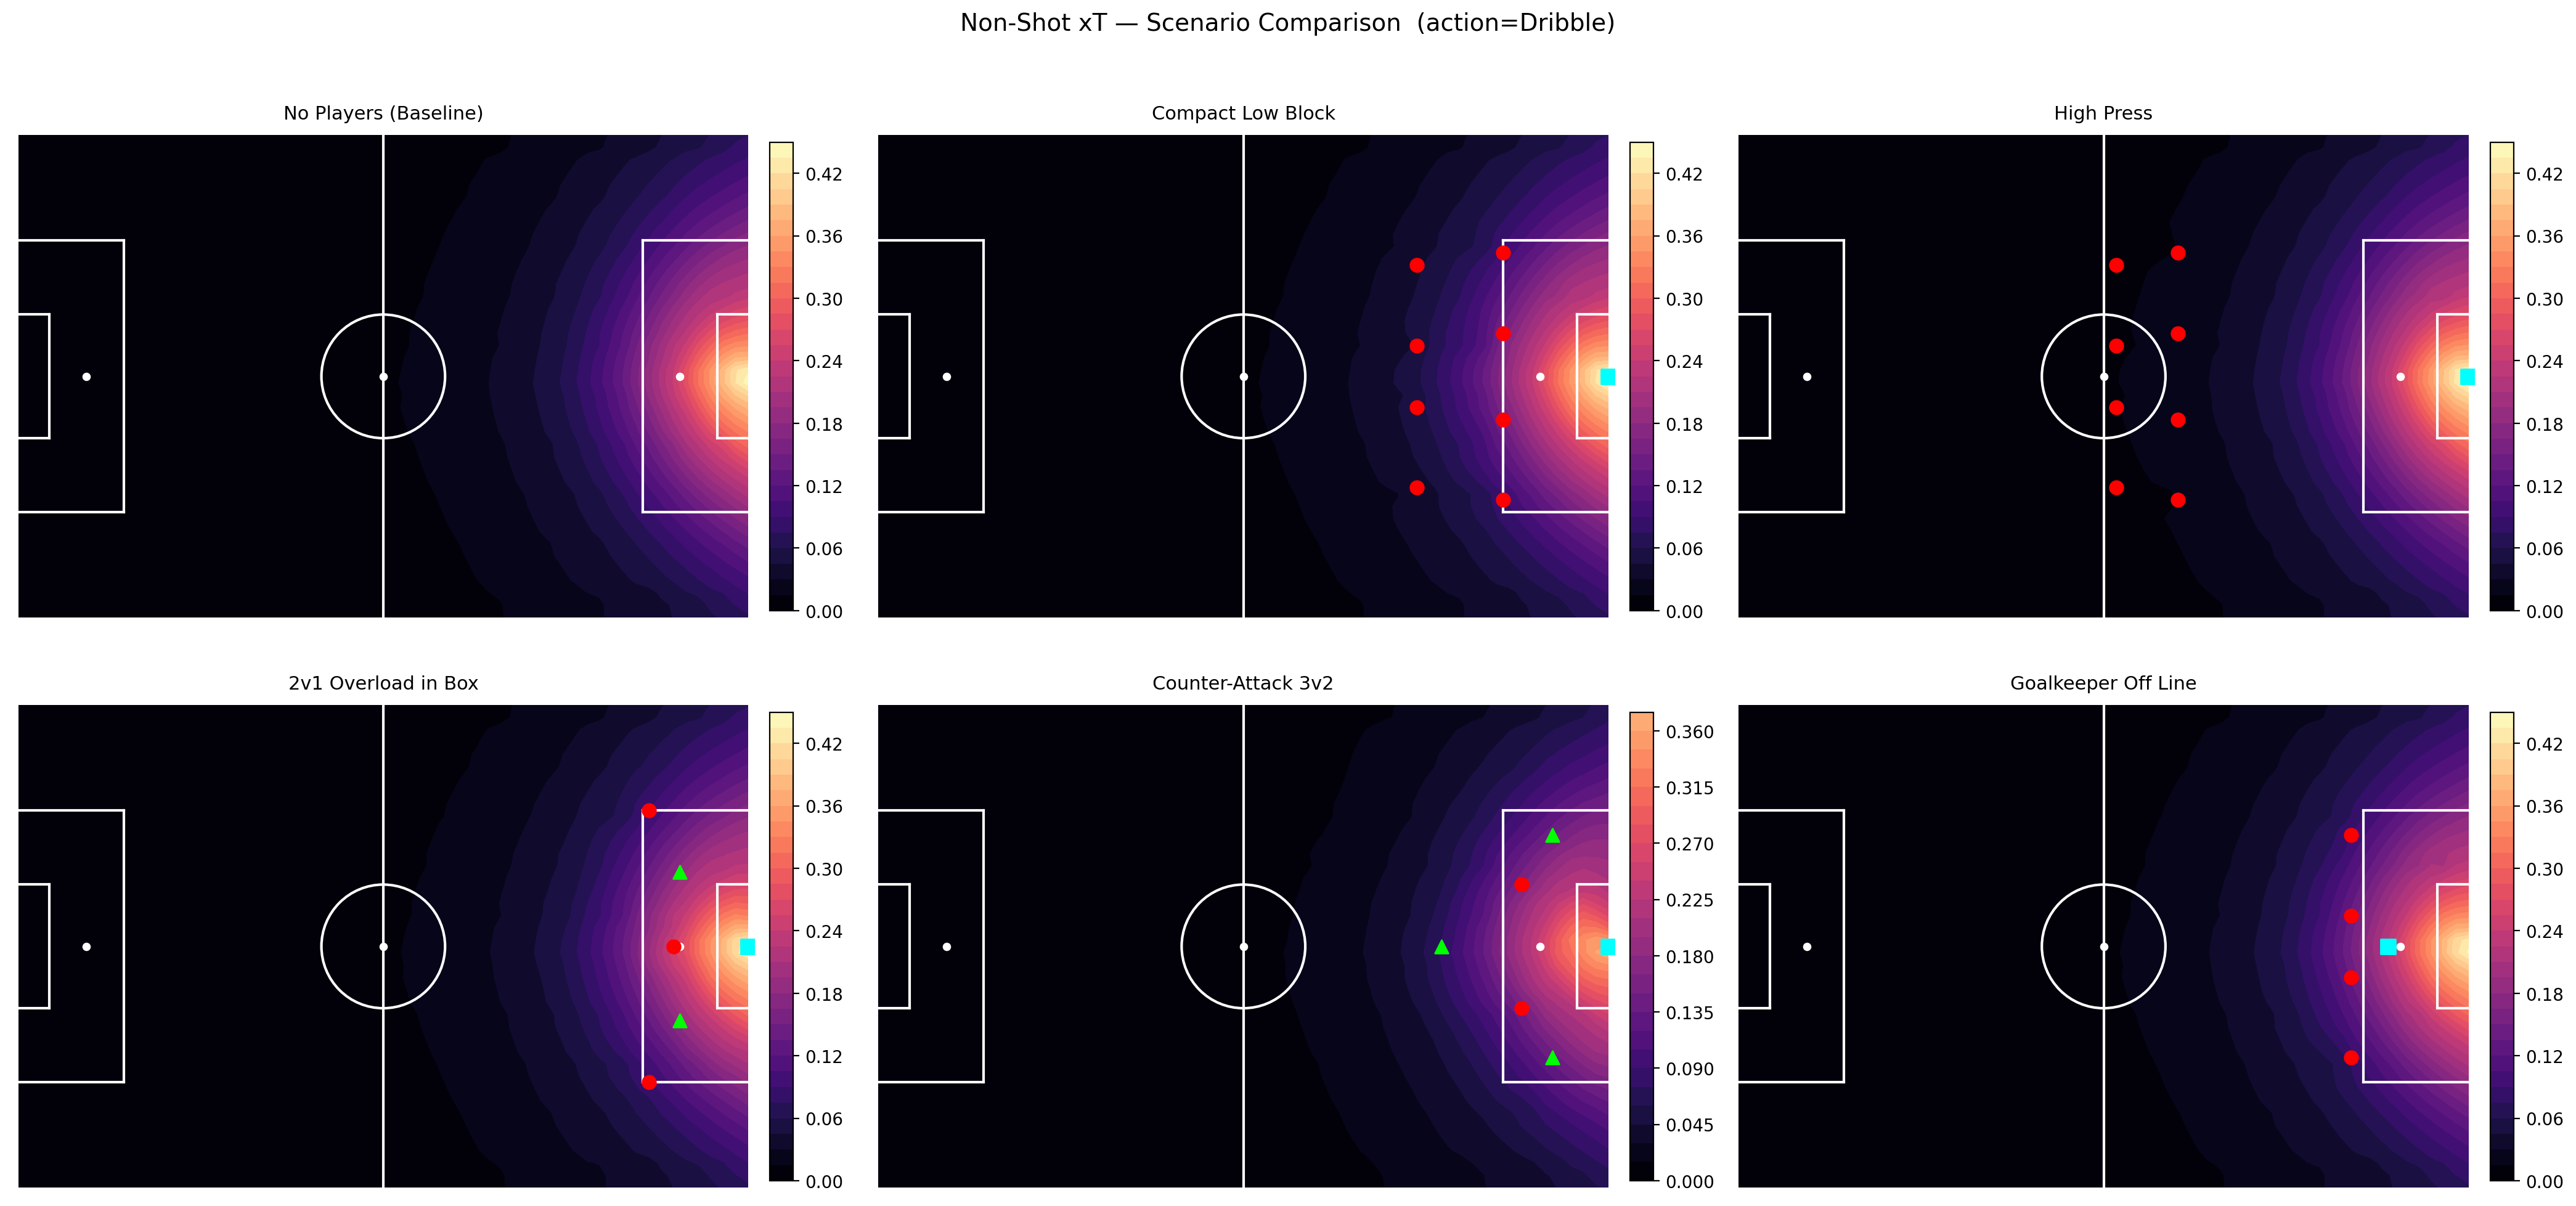
\includegraphics[width=0.8\textwidth]{../visualisations/xt_scenarios_dribble_v2.png}
    \caption{Version 2 scenario comparison, Dribble action type. End position is the ball position itself (no advancement), matching the StatsBomb training convention. Surfaces remain near-identical across formations, consistent with Version 2's structural inability to reason about individual player positions.}
    \label{fig:v2_scenarios_dribble}
\end{figure}

\section{Version 3: Transformer}

\begin{figure}[h]
\centering
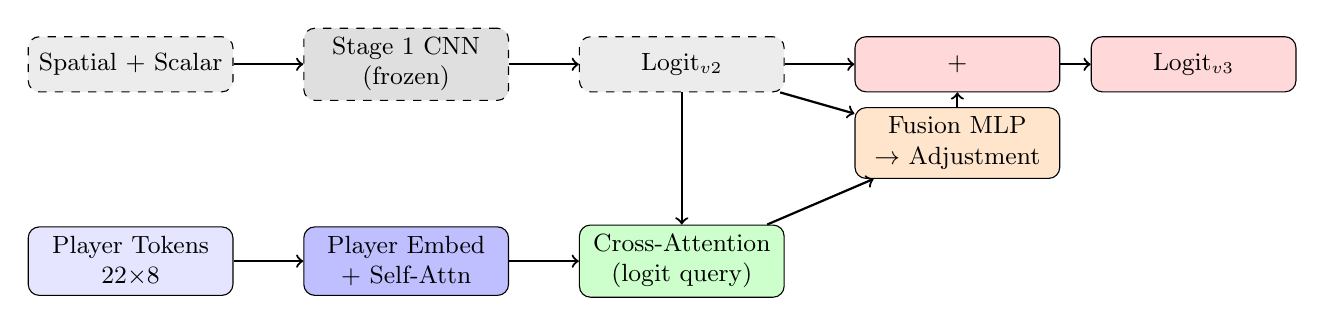
\begin{tikzpicture}[
    box/.style={draw, rounded corners, minimum width=2.6cm, minimum height=0.7cm, align=center, font=\small},
    frozen/.style={draw, rounded corners, minimum width=2.6cm, minimum height=0.7cm, align=center, font=\small, dashed},
    arr/.style={->, thick}
]
\node[frozen, fill=gray!15]  (sp)     at (0, 4)    {Spatial + Scalar};
\node[frozen, fill=gray!25]  (v2)     at (3.5, 4)  {Stage 1 CNN\\(frozen)};
\node[frozen, fill=gray!15]  (logit1) at (7, 4)    {Logit$_{v2}$};

\node[box, fill=blue!10]  (ptok)   at (0, 1.5)  {Player Tokens\\$22{\times}8$};
\node[box, fill=blue!25]  (embed)  at (3.5, 1.5){Player Embed\\+ Self-Attn};
\node[box, fill=green!20] (cross)  at (7, 1.5)  {Cross-Attention\\(logit query)};
\node[box, fill=orange!20](fusion) at (10.5,3)  {Fusion MLP\\$\to$ Adjustment};

\node[box, fill=red!15]   (add)    at (10.5, 4) {$+$};
\node[box, fill=red!15]   (out)    at (13.5, 4) {Logit$_{v3}$};

\draw[arr] (sp)     -- (v2);
\draw[arr] (v2)     -- (logit1);
\draw[arr] (logit1) -- (add);
\draw[arr] (ptok)   -- (embed);
\draw[arr] (embed)  -- (cross);
\draw[arr] (logit1) -- (cross);
\draw[arr] (cross)  -- (fusion);
\draw[arr] (logit1) -- (fusion);
\draw[arr] (fusion) -- (add);
\draw[arr] (add)    -- (out);
\end{tikzpicture}
\caption{Version 3 two-stage architecture. The frozen Stage 1 CNN (dashed) produces a baseline logit. Stage 2 encodes player tokens through self-attention (left branch); the Stage 1 logit is projected to a query vector that attends over the player context via cross-attention. The attended context and the Stage 1 logit are fused by the MLP to produce a scalar adjustment, which is added to the Stage 1 logit.}
\label{fig:v3arch}
\end{figure}

\begin{figure}[h]
    \centering
    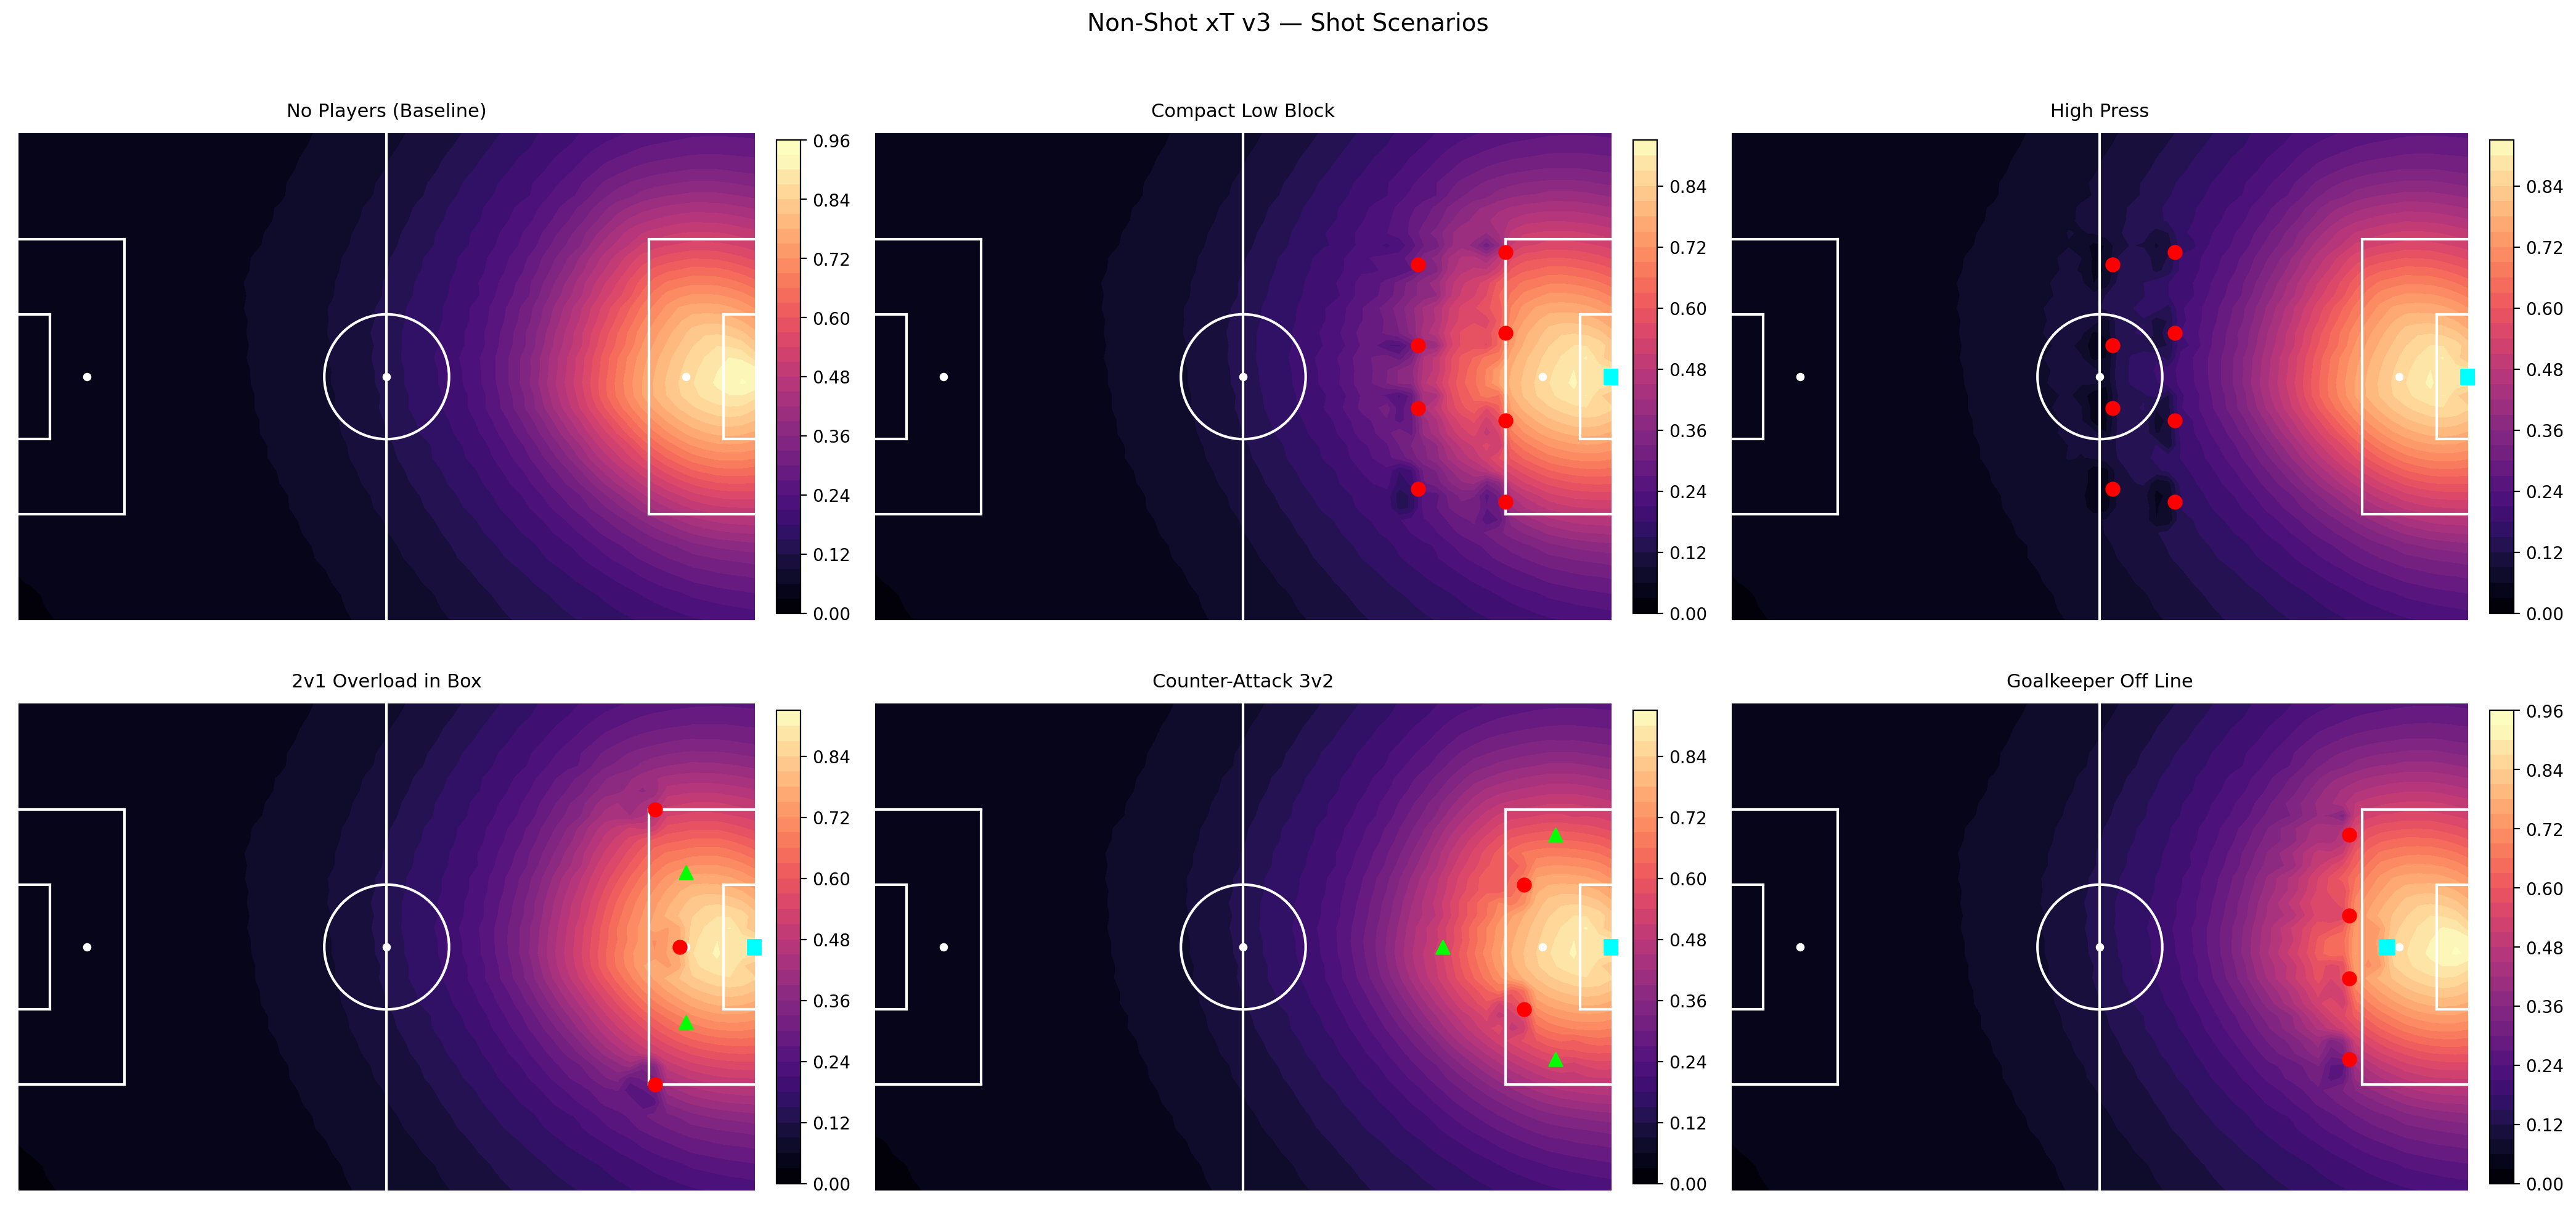
\includegraphics[width=0.8\textwidth]{../visualisations/xt_scenarios_shot_v3.png}
    \caption{Scenario comparison for Version 3, Shot action type. The first panel (no players) serves as the positional baseline. Different defensive formations produce visibly distinct threat landscapes --- a qualitative contrast to the near-identical Version 2 panels. These are illustrative inputs, not held-out measurements; the ablation (Section~\ref{sec:v3_ablation}) quantifies the player-token contribution on held-out data.}
    \label{fig:v3_scenarios}
\end{figure}

\label{sec:v3_scenarios_appendix}
The following figures show Version 3 scenario grids for Pass, Carry, and Dribble. The Pass black-panel convention (zero xT when no outfield teammates are present) is the same as for Version 2 above. For scenarios with teammates, Version 3 evaluates each teammate's position as a pass target and shows the maximum xT, using the per-player token representation of the Transformer.

\begin{figure}[h]
    \centering
    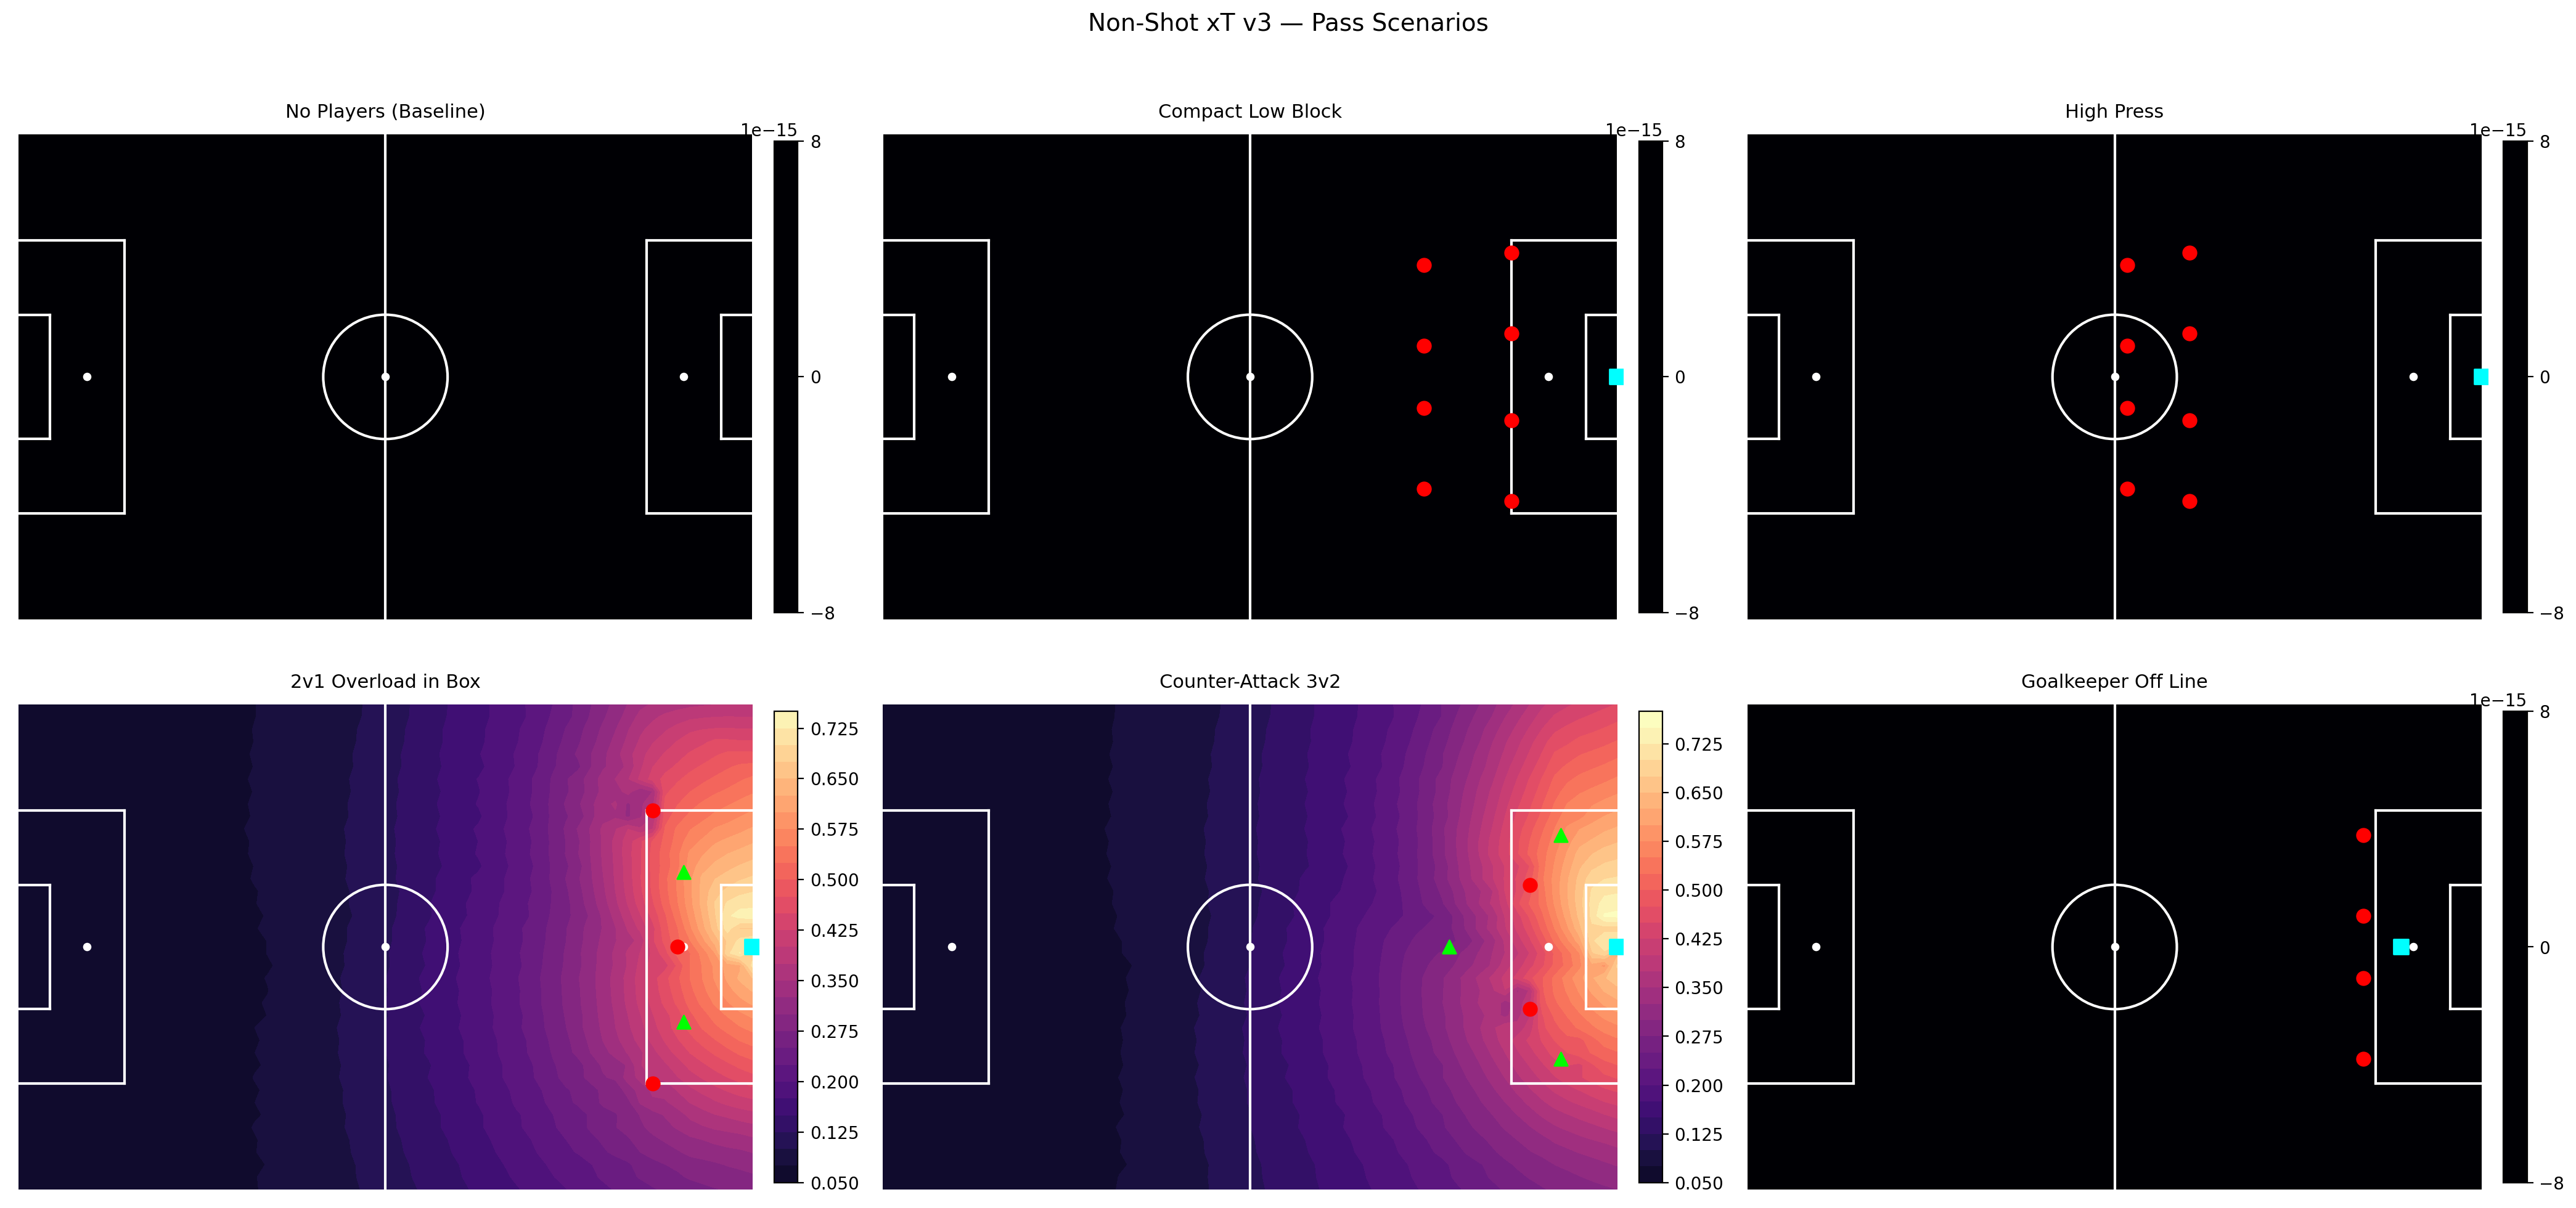
\includegraphics[width=0.8\textwidth]{../visualisations/xt_scenarios_pass_v3.png}
    \caption{Version 3 scenario comparison, Pass action type. Panels without outfield teammates are black by design. The 2v1 Overload and Counter-Attack panels show elevated Pass threat where the Transformer recognises the positioning of teammates relative to defenders, producing non-uniform threat surfaces that differ from the Version 2 equivalents.}
    \label{fig:v3_scenarios_pass}
\end{figure}

\begin{figure}[h]
    \centering
    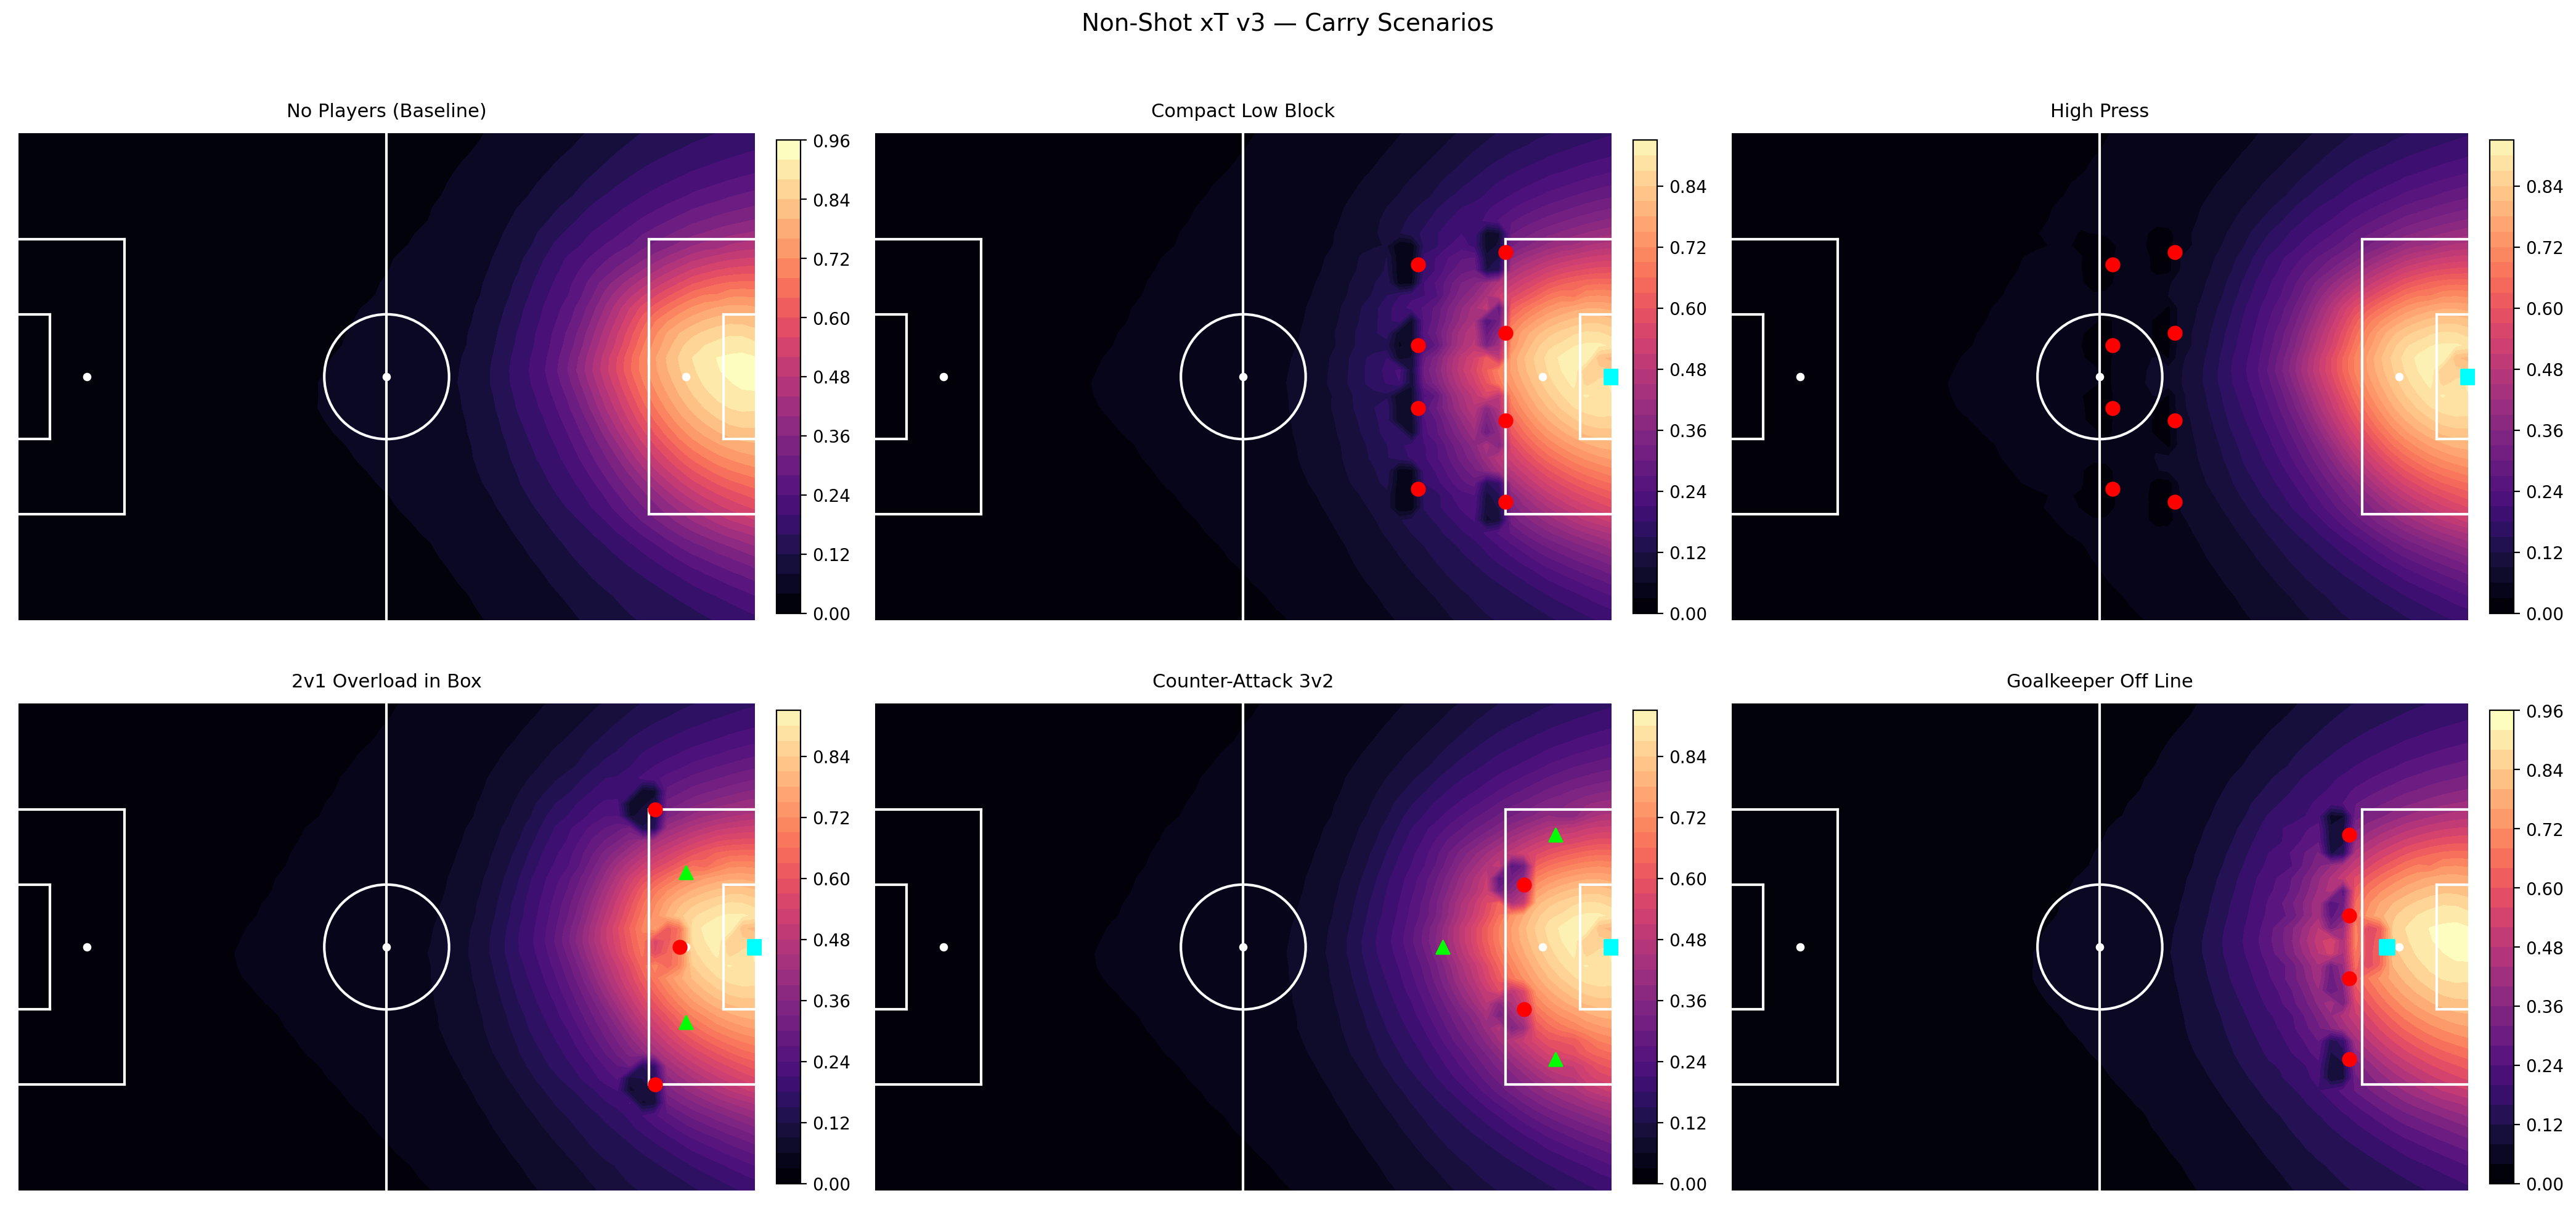
\includegraphics[width=0.8\textwidth]{../visualisations/xt_scenarios_carry_v3.png}
    \caption{Version 3 scenario comparison, Carry action type. End position is inferred as 8 yards toward goal from each cell. Unlike Version 2, the Transformer produces formation-sensitive surfaces: the Compact Low Block and High Press scenarios yield visibly different patterns, reflecting the model's ability to reason about individual defender positions relative to the carry path.}
    \label{fig:v3_scenarios_carry}
\end{figure}

\begin{figure}[h]
    \centering
    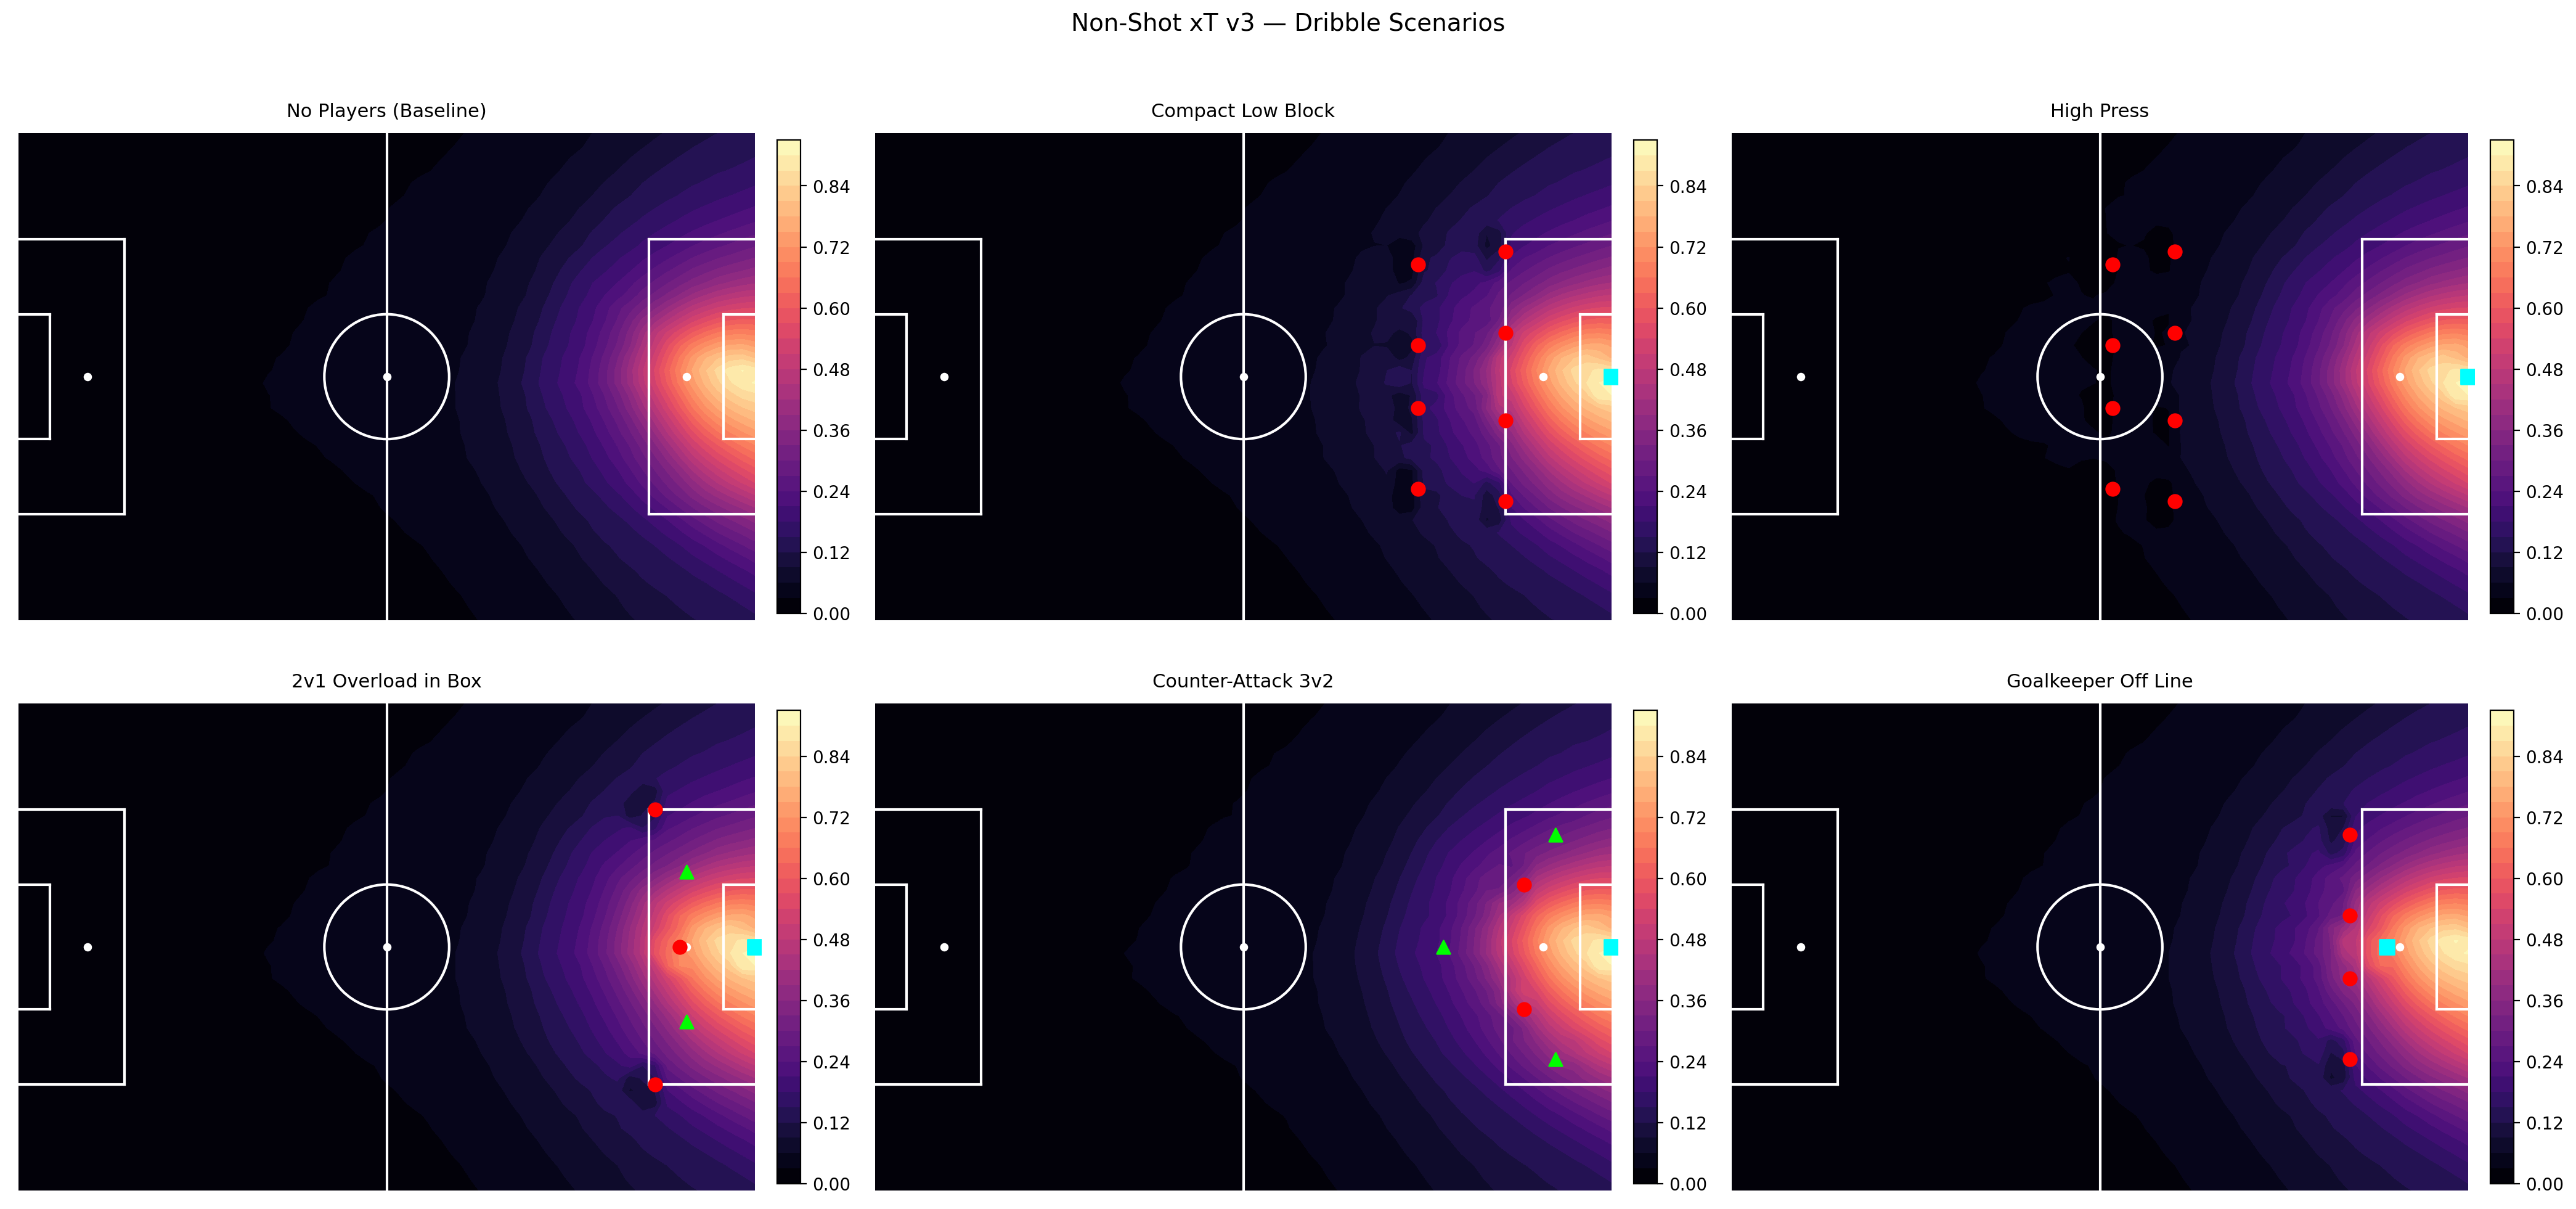
\includegraphics[width=0.8\textwidth]{../visualisations/xt_scenarios_dribble_v3.png}
    \caption{Version 3 scenario comparison, Dribble action type. End position is the ball position itself (no advancement). The Transformer's player-token representation allows it to modulate threat based on how many defenders are immediately goalside of the ball carrier, producing formation-sensitive outputs absent from Version 2.}
    \label{fig:v3_scenarios_dribble}
\end{figure}

\clearpage

\section{Interactive Frontend}

\begin{figure}[h]
    \centering
    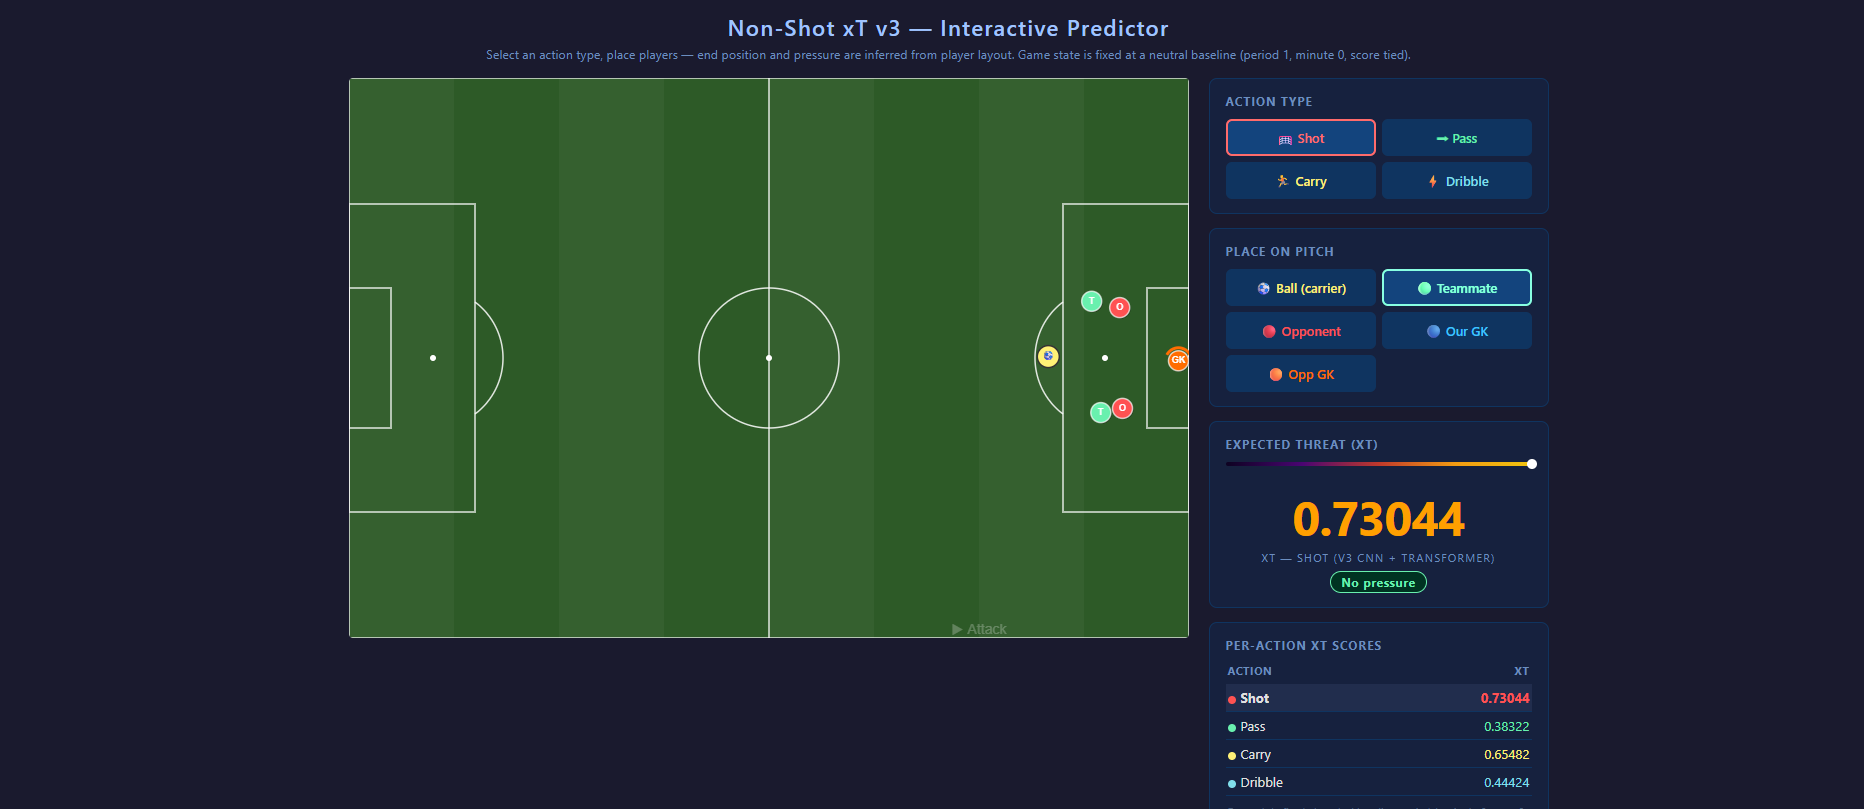
\includegraphics[width=\textwidth]{../visualisations/frontend_screenshot.png}
    \caption{Interactive xT web frontend: ball carrier placed near the edge of the penalty area with teammates and opponents in the box. The Shot action type is selected; the model returns an xT of 0.73044 for a shot from this position with this player layout. The per-action table alongside shows all four action scores simultaneously. Game state is fixed at a neutral baseline (period 1, minute 0, score tied).}
    \label{fig:frontend}
\end{figure}
